\chapter{Perturbation, KAM, And Breakdown Of Invariant Tori}
\label{chap:perturbation-chaos}

\section{From Integrable Motion To Transport}
\label{sec:perturbation-chapter-purpose}

A massless asteroid orbits the Sun while Jupiter perturbs it. Without Jupiter,
the problem is Kepler motion, one of the most integrable systems in classical
mechanics. After Jupiter is included, resonances appear, invariant tori
fragment, and transport channels open. The full restricted three-body
formulation, including
Lagrange points and ejection statistics, is developed separately in
Chapter~\ref{chap:three-body-problem}.

This question changed the meaning of ``solving'' a mechanical system. The
nineteenth-century hope was that enough first integrals would reduce the motion
to quadratures. Poincare's 1890 negative theorem showed that generic
perturbations of an integrable Hamiltonian need not admit additional analytic
first integrals beyond the energy; his later work on the three-body problem
exposed the stable-unstable manifold tangles behind this failure. Kolmogorov,
Arnold, and Moser then identified the survival theorem inside the failure:
sufficiently irrational invariant tori persist, while resonant regions become
the sites of islands, separatrix splitting, and transport. The standard map is
this chapter's compact laboratory; the asteroid problem is the gravitational
setting we revisit once the perturbative mechanisms are clear.

The precise Poincare statement is not that no special integral can ever occur.
It is a generic obstruction theorem. In lecture-note form: for a nondegenerate
integrable Hamiltonian \(H_0(I)\) and a generic analytic perturbation
\(H_0+\eps H_1\), there is no additional first integral analytic in
\((I,\theta,\eps)\), independent of the Hamiltonian, and reducing at
\(\eps=0\) to a genuinely new integral on the resonant region. The circular
restricted three-body problem realizes this obstruction physically: the Jacobi
constant survives, but one should not expect a second analytic integral that
restores two-degree-of-freedom integrability.

\begin{assumption}[Celestial perturbation model]
When a celestial example is needed, this chapter uses a planar restricted
model:
\begin{enumerate}
\item the Sun has mass \(M_\odot\);
\item Jupiter has mass \(M_J\) and follows a prescribed circular orbit;
\item asteroids are massless test particles;
\item asteroid-asteroid interactions are neglected;
\item all motion is confined to one plane.
\end{enumerate}
This model is a controlled Hamiltonian laboratory for perturbation, resonance,
and transport. It is not intended as a high-precision Solar System ephemeris.
\end{assumption}

\paragraph{Roadmap.}
The chapter uses Kepler motion as the integrable reference, canonical
perturbation theory to expose small divisors, KAM theory for torus survival,
and resonance geometry for torus breakdown.

Appendix~\ref{app:kam-proof-architecture} gives the more technical proof
architecture behind the KAM statement used here: analytic domains, the
homological equation, twist and isoenergetic variants, small-divisor estimates,
and the Cantor-measure conclusion. The present chapter keeps those estimates at
the level needed to understand the mechanics.

Three levels run through the discussion. The analytic level asks whether a
near-identity canonical transformation can remove angle dependence. The
geometric level asks which invariant tori, islands, and separatrices organize
phase space. The numerical level asks how an ensemble moves through that
geometry over a finite time. The asteroid ejection experiment in the next
chapter is meaningful only because these levels explain where transport
channels come from.

\paragraph{How approximations are labelled.}
Perturbation theory is useful only when the bookkeeping is explicit. In this
chapter \(H_0\) denotes the exactly integrable reference problem, \(\eps H_1\)
denotes a controlled perturbation, \(O(\eps^2)\) denotes terms dropped by a
first-order calculation, and resonance conditions such as \(k\cdot\omega=0\)
identify where that first-order calculation is least trustworthy. Numerical
experiments later in the chapter test the transport suggested by these
estimates over a stated finite time horizon.

\section{Kepler Motion As The Integrable Reference}
\label{sec:kepler-perturbation}

For two bodies of masses \(m_1,m_2\), let
\[
  r=x_1-x_2
\]
be the relative position and
\[
  \mu=\frac{m_1m_2}{m_1+m_2}
\]
the reduced mass. The relative Hamiltonian is
\[
  H(r,p)=\frac{\norm{p}^2}{2\mu}-\frac{Gm_1m_2}{\norm r}.
\]
For a massless asteroid around the Sun, we divide by asteroid mass and work
with the specific Hamiltonian
\[
  h(r,v)=\frac12\norm v^2-\frac{GM_\odot}{r},
  \qquad r=\norm r.
\]

\paragraph{Local notation.}
The vector \(r\) is the relative position, while \(r=\norm r\) denotes its
length after the formula is reduced to a radial expression.  The reduced mass
\(\mu\) belongs to the two-body Hamiltonian, whereas the later symbol
\(\mu_\odot=GM_\odot\) is the solar gravitational parameter in a
per-unit-mass asteroid model.

\begin{derivation}[Kepler orbit equation]
The angular momentum per unit mass is
\[
  \ell=r^2\dot\theta.
\]
This \(\ell\) is the specific angular momentum. In
Chapter~\ref{chap:lagrangian}, the two-body Kepler derivation used the massful
angular momentum \(\ell_{\mathrm{mass}}=\mu r^2\dot\theta\); the two symbols
differ by the reduced mass because this chapter has divided the Hamiltonian by
the asteroid mass. Section~\ref{subsec:detailed-binet} gives the same Binet
equation with an arbitrary particle mass \(m\); setting \(m=1\) gives the
specific convention used here.
For a central potential, \(\ell\) is conserved. The radial equation is
\[
  \ddot r-r\dot\theta^2=-\frac{GM_\odot}{r^2}.
\]
Set \(u=1/r\). Using
\[
  \frac{\dd}{\dd t}=\dot\theta\frac{\dd}{\dd\theta}
  =
  \ell u^2\frac{\dd}{\dd\theta},
\]
the radial equation loses its explicit time dependence and becomes Binet's
equation for the orbit shape:
\[
  \frac{\dd^2u}{\dd\theta^2}+u=\frac{GM_\odot}{\ell^2}.
\]
Therefore
\[
  u(\theta)=\frac{GM_\odot}{\ell^2}\left(1+e\cos(\theta-\varpi)\right),
\]
equivalently
\[
  \boxed{
  r(\theta)=\frac{a(1-e^2)}{1+e\cos(\theta-\varpi)}
  }.
\]
Here \(a\) is the semimajor axis, \(e\) is eccentricity, and \(\varpi\) is the
longitude of periapse.
\end{derivation}

Bound Kepler orbits have energy
\[
  h=-\frac{GM_\odot}{2a}.
\]
Kepler's third law follows from the period \(T\):
\[
  n^2a^3=GM_\odot,\qquad n=\frac{2\pi}{T}.
\]

\section{Action-Angle View Of Kepler Motion}
\label{sec:kepler-action-angle}

The Kepler problem is more than solvable; it is superintegrable. For
perturbation theory, the most useful idea is that unperturbed motion can be
written in action-angle form:
\[
  H_0=H_0(I),
  \qquad
  \dot I=0,
  \qquad
  \dot\theta=\omega(I).
\]

\paragraph{Local notation.}
Here \(I\) denotes a vector of action variables and \(\theta\) denotes the
corresponding angle variables.  These are not the rigid-body inertia tensor and
not the Euler polar angle.  The frequency vector is
\(\omega(I)=\partial H_0/\partial I\).

For a near-integrable Hamiltonian,
\[
  H(I,\theta)=H_0(I)+\eps H_1(I,\theta),
\]
the actions are no longer exactly constant:
\[
  \dot I=-\eps\frac{\partial H_1}{\partial \theta},
  \qquad
  \dot\theta=\frac{\partial H_0}{\partial I}
  +
  \eps\frac{\partial H_1}{\partial I}.
\]
The small parameter \(\eps\) should be interpreted physically. In the
Sun-Jupiter-asteroid problem, a natural scale is \(M_J/M_\odot\), though close
encounters and resonances can amplify its effect.

\section{Planar Delaunay And Poincare Variables}
\label{sec:planar-delaunay-poincare}

The previous section described action-angle variables abstractly.  Celestial
mechanics needs a concrete version for Kepler ellipses, because resonances are
defined by combinations of orbital phases.  In this section the symbol
\[
  \mu_\odot=GM_\odot
\]
denotes the solar gravitational parameter.  This is not the reduced mass; it is
the parameter that appears in the specific Kepler Hamiltonian
\[
  h_0(r,v)=\frac12\norm v^2-\frac{\mu_\odot}{r}.
\]
The specific energy of a bound orbit is
\[
  h_0=-\frac{\mu_\odot}{2a}.
\]
The action conjugate to the fast Kepler phase is
\[
  \boxed{\Lambda=\sqrt{\mu_\odot a}.}
\]
This normalization is fixed by the Kepler action integral, not by dimensional
guesswork.  For a planar ellipse with angular-momentum action
\(G_{\rm D}=\sqrt{\mu_\odot a(1-e^2)}\), the radial action is
\[
  J_r
  =
  \frac{1}{2\pi}\oint p_r\,\dd r
  =
  \sqrt{\mu_\odot a}-G_{\rm D}.
\]
The action conjugate to the mean anomaly is the sum
\(J_r+G_{\rm D}\), because the radial oscillation and angular advance combine
into one closed Kepler period.  Thus \(J_r+G_{\rm D}=\sqrt{\mu_\odot a}\),
which is the \(\Lambda\) displayed above.  The longer calculation below keeps
\(J_r\) explicit in order to introduce the eccentricity action.
Solving for \(a=\Lambda^2/\mu_\odot\) gives
\[
  \boxed{
  H_0(\Lambda)=-\frac{\mu_\odot^2}{2\Lambda^2}.
  }
\]
Therefore the Kepler mean motion is
\[
  \dot\lambda=\frac{\partial H_0}{\partial \Lambda}
  =
  \frac{\mu_\odot^2}{\Lambda^3}
  =
  \sqrt{\frac{\mu_\odot}{a^3}},
\]
which is exactly Kepler's third law.

\begin{derivation}[Radial action and the second planar Delaunay action]
In the planar Kepler problem the angular momentum per unit mass is
\[
  G_{\rm D}=\sqrt{\mu_\odot a(1-e^2)}.
\]
The subscript reminds us that \(G_{\rm D}\) is the Delaunay angular-momentum
action; it is not Newton's gravitational constant.  The radial momentum is
determined by the energy equation
\[
  \frac12 p_r^2+\frac{G_{\rm D}^2}{2r^2}-\frac{\mu_\odot}{r}
  =
  -\frac{\mu_\odot}{2a}.
\]
The radial action is
\[
  J_r=\frac{1}{2\pi}\oint p_r\,\dd r .
\]
For a Kepler ellipse this integral evaluates to
\[
  J_r
  =
  \sqrt{\mu_\odot a}-\sqrt{\mu_\odot a(1-e^2)}
  =
  \Lambda-G_{\rm D}.
\]
Thus the two planar actions may be taken as \(\Lambda\) and \(G_{\rm D}\), or
equivalently as \(\Lambda\) and
\[
  \Gamma=\Lambda-G_{\rm D}.
\]
For small eccentricity,
\[
  \Gamma
  =
  \Lambda\left(1-\sqrt{1-e^2}\right)
  =
  \frac12\Lambda e^2+O(e^4).
\]
The action \(\Gamma\) is therefore the eccentricity action: it vanishes on a
circular orbit and grows quadratically with \(e\).
\end{derivation}

Let \(M\) be the mean anomaly and let \(\varpi\) be the longitude of
periapse.  The symbol \(M\) is used here to avoid conflict with the specific
angular momentum \(\ell=r^2\dot\theta\) used in the preceding Kepler
derivation.  Planar Delaunay coordinates are
\[
  (\Lambda,M),\qquad (G_{\rm D},\varpi),
\]
with canonical one-form
\[
  \Lambda\,\dd M+G_{\rm D}\,\dd\varpi .
\]
Since \(H_0\) depends only on \(\Lambda\),
\[
  \dot M=\frac{\partial H_0}{\partial \Lambda},
  \qquad
  \dot\varpi=\frac{\partial H_0}{\partial G_{\rm D}}=0.
\]
This is the Kepler degeneracy.  The periapse does not precess in the ideal
two-body problem, so the frequency map is degenerate in the full set of
Delaunay actions.  Celestial KAM theory therefore cannot be applied to the pure
Kepler problem by simply quoting the nondegenerate theorem from
Section~\ref{sec:kam-theorem-sketch}; one first needs the secular structure
created by interactions, averaging, or additional degrees of freedom.

For perturbations near circular orbits, \(\varpi\) is a poor coordinate because
the direction of periapse is undefined when \(e=0\).  Poincare variables remove
this artificial singularity.  Define the mean longitude and eccentricity angle
by
\[
  \lambda=M+\varpi,\qquad \gamma=-\varpi,
\]
and keep
\[
  \Gamma=\Lambda-G_{\rm D}.
\]
Then
\[
  \Lambda\,\dd M+G_{\rm D}\,\dd\varpi
  =
  \Lambda\,\dd\lambda+\Gamma\,\dd\gamma,
\]
so \((\Lambda,\lambda)\) and \((\Gamma,\gamma)\) are canonical pairs.  Finally
set
\[
  x=\sqrt{2\Gamma}\cos\gamma,\qquad
  y=\sqrt{2\Gamma}\sin\gamma.
\]
The pair \((x,y)\) is a Cartesian representation of the eccentricity degree of
freedom.  The origin \((x,y)=(0,0)\) is the circular orbit; no angle has to be
chosen there.

\begin{figure}[htbp]
\centering
\begin{tikzpicture}[x=1cm,y=1cm, >=Latex, font=\small]
  \begin{scope}
    \draw[->] (-2.0,0) -- (2.2,0) node[right] {major axis};
    \draw[->] (0,-1.45) -- (0,1.65) node[above] {minor axis};
    \draw[blue!70!black, thick, rotate=18] (0,0) ellipse (1.65 and 0.86);
    \fill[yellow!80!black] (-0.55,0) circle (2.5pt)
      node[below=4pt, fill=white, inner sep=1pt] {Sun};
    \fill[blue!70!black] (0.98,0.56) circle (1.8pt)
      node[above right, fill=white, inner sep=1pt] {asteroid};
    \draw[red!75!black, ->, thick] (0,0) -- (1.56,0.51)
      node[midway, above, fill=white, inner sep=1pt] {\(\varpi\)};
    \draw[green!45!black, ->, thick] (0,0) -- (0.98,0.56)
      node[midway, below right, fill=white, inner sep=1pt] {\(\lambda\)};
    \node[align=center] at (0,-1.85)
      {ellipse: size \(a\), shape \(e\),\\phase \(\lambda\), periapse \(\varpi\)};
  \end{scope}
  \begin{scope}[xshift=6.0cm]
    \draw[->] (-1.6,0) -- (1.8,0) node[right] {\(x\)};
    \draw[->] (0,-1.45) -- (0,1.65) node[above] {\(y\)};
    \draw[blue!35, fill=blue!6] (0,0) circle (1.02);
    \draw[red!75!black, ->, thick] (0,0) -- (0.72,0.72)
      node[midway, above left, fill=white, inner sep=1pt] {\(\sqrt{2\Gamma}\)};
    \draw[gray!70, ->] (0.55,0) arc (0:45:0.55);
    \node[gray!50!black, fill=white, inner sep=1pt] at (0.82,0.24) {\(\gamma\)};
    \fill[blue!70!black] (0,0) circle (2pt)
      node[below left, fill=white, inner sep=1pt] {\(e=0\)};
    \node[align=center] at (0,-1.85)
      {Poincare eccentricity plane:\\\(\Gamma\approx\Lambda e^2/2\)};
  \end{scope}
\end{tikzpicture}
\caption{Planar Poincare variables replace the singular periapse angle at
\(e=0\) by Cartesian eccentricity coordinates.  The action \(\Lambda\)
measures semimajor axis, while \(\Gamma\) measures eccentricity to leading
order.}
\label{fig:delaunay-poincare-variables}
\end{figure}

\section{Resonance}
\label{sec:resonance}

\begin{definition}[Resonance]
A resonance occurs when there is a nonzero integer vector \(k\in\Z^n\) such
that
\[
  k\cdot\omega(I)=0.
\]
Near resonance, phase combinations that normally average out become slow and
can accumulate over long times.
\end{definition}

\paragraph{Local notation.}
The vector \(k\) labels an integer Fourier mode or integer frequency
combination.  In celestial mean-motion resonances, the symbols \(p:q\) label
the ratio of mean motions \(n/n_J\); they are resonance integers, not canonical
momenta.

For mean-motion resonance with Jupiter, a \(p:q\) resonance means
\[
  \frac{n}{n_J}\approx \frac{p}{q}.
\]
Using Kepler's law,
\[
  \frac{n}{n_J}\approx
  \left(\frac{a_J}{a}\right)^{3/2},
\]
so the nominal resonance location is
\[
  \boxed{
  a_{p:q}=a_J\left(\frac{q}{p}\right)^{2/3}
  }.
\]
This formula is only the center of a resonance zone. The width of the zone
depends on the perturbation strength, eccentricity, and the order of the
resonance. The point of marking the nominal location is to identify where slow
angle combinations can form; the later chaos discussion explains what happens
inside and near those zones.
The missing-asteroid bands at these resonances are the Kirkwood gaps,
identified empirically by Daniel Kirkwood in 1866 before modern Hamiltonian
perturbation theory supplied the phase-space explanation.

In the planar Sun-Jupiter-asteroid model, let
\[
  \lambda_J=n_Jt+\lambda_{J,0}
\]
be Jupiter's mean longitude.  For an interior \(p:q\) resonance, with
\(p>q\) and \(n/n_J\approx p/q\), the lowest-order eccentricity-type resonant
angle is
\[
  \boxed{
  \phi_{p:q}
  =
  p\lambda_J-q\lambda-(p-q)\varpi .
  }
\]
The coefficient of \(\varpi\) is forced by rotational invariance: adding a
constant angle to all longitudes must leave the phase unchanged.  Differentiating
gives
\[
  \dot\phi_{p:q}
  =
  pn_J-qn-(p-q)\dot\varpi .
 \]
At exact Keplerian commensurability \(qn=pn_J\), and in the unperturbed Kepler
problem \(\dot\varpi=0\), so this angle is slow.  The resonant perturbation
depends on a slow phase and therefore does not average away.

For the low-order interior Jovian resonances used in the demos,
\[
\begin{array}{ccl}
3:1 &:& \phi=3\lambda_J-\lambda-2\varpi,\\
5:2 &:& \phi=5\lambda_J-2\lambda-3\varpi,\\
7:3 &:& \phi=7\lambda_J-3\lambda-4\varpi,\\
2:1 &:& \phi=2\lambda_J-\lambda-\varpi .
\end{array}
\]
The order of the eccentricity-type term is \(p-q\).  Thus the \(3:1\) term is
second order in eccentricity, the \(5:2\) term is third order, and the \(2:1\)
term is first order.  This order statement is a scaling statement, not a full
disturbing-function calculation.

\begin{figure}[htbp]
\centering
\begin{tikzpicture}[x=0.72cm,y=1cm, >=Latex, font=\small]
  \draw[->] (0,0) -- (13.8,0) node[right] {\(a\) [AU]};
  \foreach \x/\lab in {0/2.0,2/2.5,4/3.0,6/3.5,8/4.0,10/4.5,12/5.0}
    \draw (\x,0.07) -- (\x,-0.07) node[below] {\lab};
  \draw[ultra thick, blue!35] (0.1,0) -- (7.0,0);
  \node[blue!60!black, fill=white, inner sep=1.5pt] at (3.6,-0.62)
    {asteroid-belt-like annulus};
  \foreach \x/\lab/\y in {2.008/3:1/1.25,3.302/5:2/1.92,3.833/7:3/1.18,5.114/2:1/1.72}
  {
    \draw[red!75!black, thick] (\x,0.18) -- (\x,0.92);
    \draw[red!75!black, thin] (\x,0.92) -- (\x,\y-0.10);
    \node[red!75!black, fill=white, inner sep=1pt] at (\x,\y) {\lab};
  }
  \fill[orange!80!black] (12.82,0) circle (2.2pt);
  \node[orange!80!black, above=3pt, fill=white, inner sep=1pt] at (12.45,0.18) {Jupiter};
\end{tikzpicture}
\caption{Nominal mean-motion resonance locations with Jupiter, shown
across an asteroid-belt-like range. The resonance positions use
\(a_{p:q}=a_J(q/p)^{2/3}\); the figure now includes Jupiter's orbital radius to
show that the listed resonances lie interior to Jupiter.}
\label{fig:jupiter-resonance-locations}
\end{figure}

\subsection{Celestial Resonant Normal Form}
\label{subsec:celestial-resonant-normal-form}

The generic resonant normal form derived later in
Section~\ref{subsec:resonant-normal-form-island-width} has a direct celestial
interpretation.  In the planar restricted problem, after introducing the
forcing phase \(\lambda_J\) and its conjugate action, write the Hamiltonian
schematically as
\[
  K(\Lambda,\Gamma,\lambda,\gamma,\lambda_J,I_J)
  =
  H_0(\Lambda)+n_JI_J
  +\eps R(\Lambda,\Gamma,\lambda,\gamma,\lambda_J),
\]
where \(\eps\) is of order \(M_J/M_\odot\) away from close encounters.  Near a
\(p:q\) resonance, perform a canonical change in which the slow angle is
\(\phi_{p:q}\).  Averaging over the remaining fast angle gives a one-degree
resonant Hamiltonian of the form
\[
  K_{\rm res}(J,\phi)
  =
  K_*
  +
  \frac12 A(J-J_*)^2
  +
  \eps B_{p:q}(\Gamma_*)\cos\phi
  +\cdots .
\]

\paragraph{Local notation.}
The action \(J\) in this subsection is the resonant action produced by the
canonical change of variables; it is unrelated to angular momentum \(J\) in the
rigid-body chapter.  The quantity \(I_J\) is the dummy action conjugate to
Jupiter's imposed phase in the autonomous extension.  The coefficient
\(B_{p:q}\) is a Fourier coefficient of the disturbing function after averaging.

Here \(J\) is the resonant action measuring displacement from the exact
commensurability, \(J_*\) is its resonant value, \(A\) is the local curvature of
the frequency mismatch, and \(B_{p:q}\) is the relevant disturbing-function
coefficient after averaging.  For an eccentricity-type resonance of order
\(r=p-q\),
\[
  B_{p:q}(\Gamma_*)=O(e_*^r)
\]
for small eccentricity, with the coefficient depending on Laplace coefficients
and on the chosen normalization.

The pendulum calculation gives the scaling
\[
  \Delta J_{\max}
  =
  2\sqrt{\frac{\eps |B_{p:q}(\Gamma_*)|}{|A|}},
\]
up to the convention used to normalize \(J\).  This formula explains why
resonance widths grow like \(\sqrt{\eps}\) but it does not by itself give a
measured Kirkwood-gap width.  A gap in the observed asteroid belt also depends
on secular resonances, multiple planets, chaotic diffusion, collisions,
Yarkovsky drift, primordial depletion, and the finite age of the Solar System.

\subsection{A First Disturbing-Function Coefficient: The Interior 2:1 Resonance}
\label{subsec:disturbing-function-2to1}

The previous paragraph used \(B_{p:q}=O(e^{p-q})\) as a scaling statement.  A
real celestial-mechanics calculation must compute the coefficient multiplying
the resonant cosine.  We do this for the first-order interior \(2:1\)
resonance, because it is the cleanest example and it appears in the asteroid
demo.

\paragraph{Local notation.}
In this subsection \(\alpha=a/a_J\) is a semimajor-axis ratio, \(e\) is the
asteroid eccentricity, \(M\) is mean anomaly, \(\lambda=M+\varpi\) is mean
longitude, and \(\varpi\) is longitude of periapse.  The calligraphic
\(\mathcal R\) is the disturbing function per unit \(Gm_J/a_J\), not a
configuration-space region.

Use units \(a_J=1\) temporarily, and write
\[
  \alpha=\frac{a}{a_J}.
\]
Jupiter is circular, with longitude \(\lambda_J\).  The asteroid has mean
longitude \(\lambda=M+\varpi\).  The heliocentric disturbing function per unit
\(Gm_J/a_J\) is
\[
  \mathcal R
  =
  \frac{1}{|r_J-r|}
  -
  r\cdot r_J ,
\]
where the second term is the indirect part in these units.  For small
eccentricity,
\[
  \frac{|r|}{a} = 1-e\cos M+O(e^2),
  \qquad
  f+\varpi=\lambda+2e\sin M+O(e^2).
\]
Let
\[
  \psi=\lambda-\lambda_J .
\]
At \(e=0\), define
\[
  Q(\psi)=1-2\alpha\cos\psi+\alpha^2,
  \qquad
  D(\psi)=Q(\psi)^{-1/2}.
\]
Differentiating the direct term with respect to the radial factor \(\rho\) and
the angular separation \(\psi\) gives
\[
  D_\rho=(\alpha\cos\psi-\alpha^2)Q^{-3/2},
  \qquad
  D_\psi=-\alpha\sin\psi\,Q^{-3/2}.
\]
The indirect term \(\alpha\rho\cos\psi\) contributes
\[
  I_\rho=\alpha\cos\psi,
  \qquad
  I_\psi=-\alpha\sin\psi .
\]
Project the first-order eccentricity variation of
\(\mathcal R=D-I\) onto
\[
  \phi=2\lambda_J-\lambda-\varpi .
\]
Setting \(\varpi=0\) after using rotational invariance, averaging over the
ignorable rotation angle leaves the one-dimensional integral below.  The factor
of two relative to the raw inner product with \(\cos\phi\) is important: it is
what converts the projection into the coefficient \(C_{2:1}\) in
\(eC_{2:1}\cos\phi\).
\[
  C_{2:1}(\alpha)
  =
  \frac{1}{2\pi}\int_0^{2\pi}
  \left[
  -\cos(2\psi)(D_\rho-I_\rho)
  +
  2\sin(2\psi)(D_\psi-I_\psi)
  \right]\dd\psi .
\]
Thus the resonant term is
\[
  \mathcal R_{2:1}
  =
  e\,C_{2:1}(\alpha)
  \cos(2\lambda_J-\lambda-\varpi)+O(e^2).
\]
For the nominal \(2:1\) location,
\[
  \alpha_*=2^{-2/3}.
\]
The Python demo evaluates the integral numerically and independently checks it
by a two-angle finite-difference projection.  In the convention above it finds
\[
  C_{2:1}(\alpha_*)\simeq -1.19049 .
\]
The sign depends on whether the Hamiltonian is written with \(+\mathcal R\) or
\(-\mathcal R\); the resonance half-width depends on \(|C_{2:1}|\).

Using the local pendulum approximation in the action \(\Lambda=\sqrt{\mu_\odot
a}\), and then converting from \(\Delta\Lambda\) to semimajor axis, gives the
classroom estimate
\[
  \Delta a_{\rm half}
  \simeq
  4a_J
  \sqrt{
    \frac{\eps |C_{2:1}| e\,\alpha_*^3}{3}
  },
  \qquad
  \eps=\frac{M_J}{M_\odot}.
\]
This formula is still an idealized resonance width: it assumes the planar
circular restricted model, small eccentricity, no close encounter, and a single
isolated resonance.  Its status is nevertheless different from the
\(\eta e^r\) model: the coefficient is now computed from the disturbing
function rather than inserted as a placeholder.

\begin{figure}[htbp]
\centering
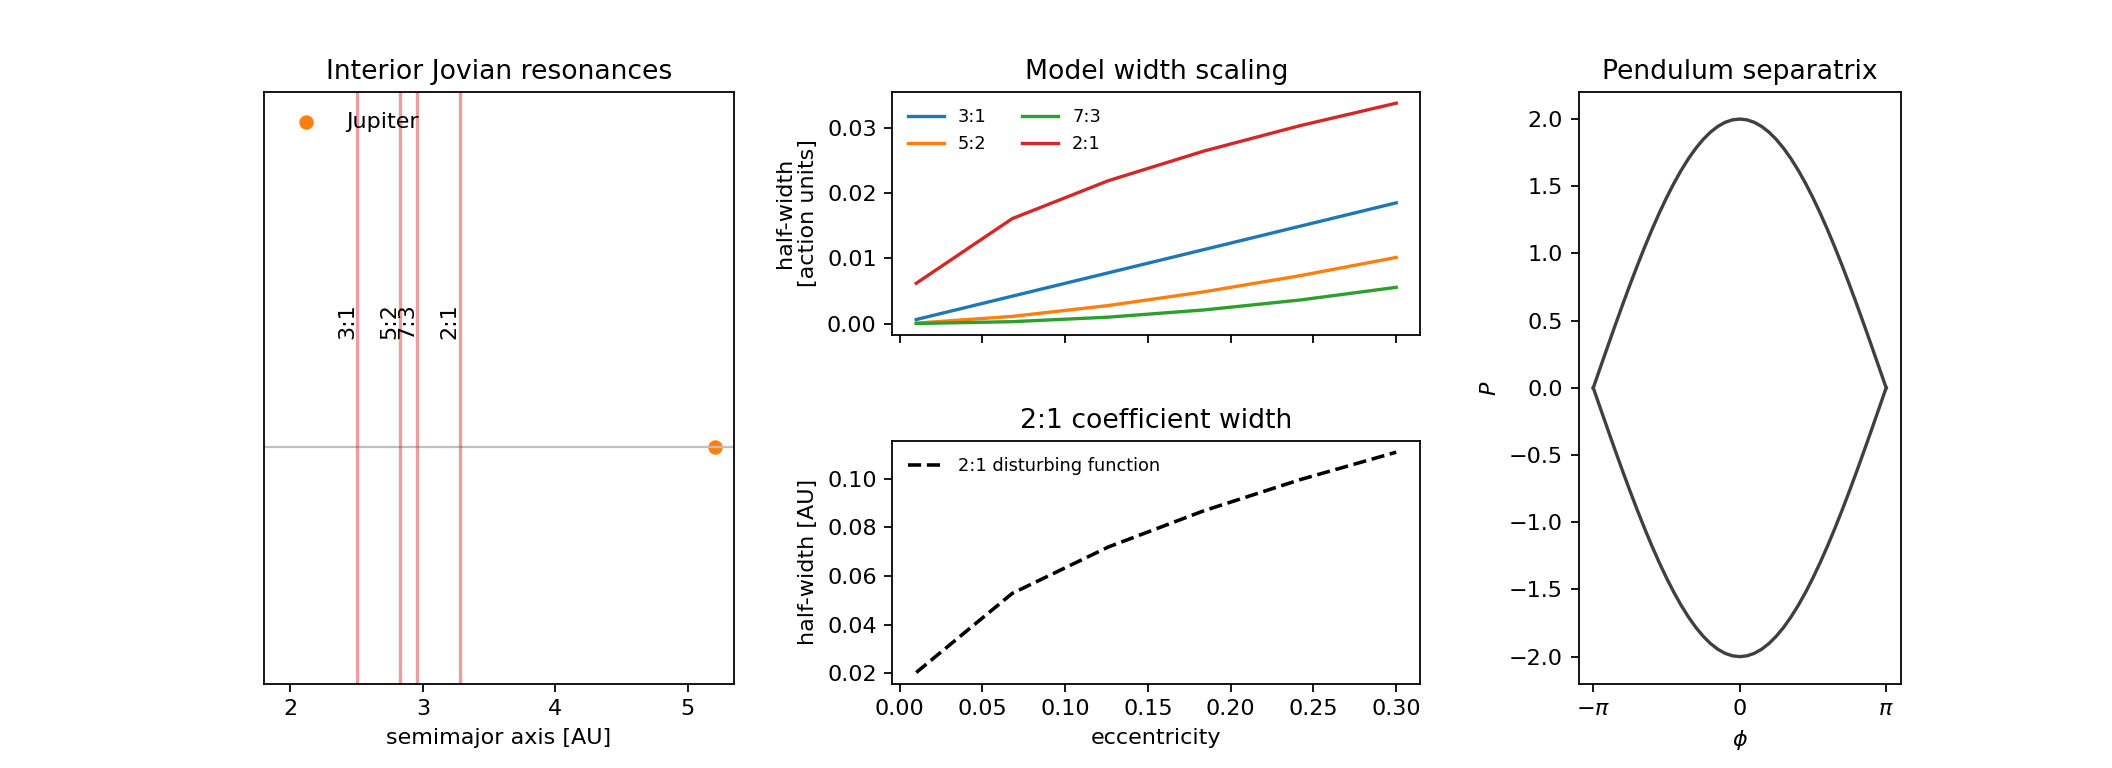
\includegraphics[width=0.98\textwidth]{../../figures/canonical/asteroid_resonance_normal_form_quick.png}
\caption{Numerical companion to the resonant normal-form calculation, generated
by \protect\path{demos/python/asteroid_resonance_normal_form.py}.  The left panel uses
semimajor axis \(a\) in astronomical units on the horizontal axis; the
vertical resonance markers are the nominal interior Jovian resonances
\(a_{p:q}=a_J(q/p)^{2/3}\), and the Jupiter marker identifies \(a_J\), not an
asteroid data point.  The two middle panels both use eccentricity \(e\) on the
horizontal axis but deliberately use different vertical scales.  The upper
middle panel shows the illustrative normal-form half-widths in dimensionless
action units for the placeholder model \(B_r(e)=\eta e^r\).  The lower middle
panel shows only the quantitative \(2:1\) half-width in astronomical units,
obtained from the disturbing-function coefficient \(C_{2:1}\) in the text.
Their heights should not be compared across panels: the separation is meant to
avoid mixing model action units with AU.  The right panel is the universal
pendulum normal form: the horizontal axis is the resonant angle
\(\phi\in[-\pi,\pi]\), the vertical axis is its conjugate momentum \(P\) in
normalized units, and the curve is the separatrix.  The panels should be read
as location, model-scaling, physical-width, and phase-portrait views of the
same resonance calculation, not as an asteroid trajectory.}
\label{fig:asteroid-resonance-normal-form-numerical}
\end{figure}

\section{Perturbing An Integrable System}
\label{sec:perturbing-integrable-system}

The central perturbation question is the following. Suppose the unperturbed
Hamiltonian is integrable and has action-angle coordinates:
\[
  H_0=H_0(I),
  \qquad
  (I,\theta)\in U\times\mathbb T^N,
  \qquad
  \dot I=0,\quad \dot\theta=\omega_0(I),
\]
where
\[
  \omega_0(I)=\frac{\partial H_0}{\partial I}.
\]
Now add a small generic perturbation:
\[
  H(I,\theta)=H_0(I)+\eps H_1(I,\theta),
  \qquad
  0<\eps\ll 1.
\]

\paragraph{Local notation.}
The domain \(U\) is an open set of actions, \(\mathbb T^N\) is the
\(N\)-torus of angles, and \(\eps\) is the dimensionless perturbation strength.
The question is local in the action-angle chart; global obstructions such as
singular tori and collisions are outside this local model.

What happens to the invariant tori \(I=\text{constant}\)?

Two tempting answers are both incomplete. One might hope that the perturbed
system remains integrable after a clever change of variables. One might also
expect that a generic perturbation destroys the tori and makes a typical orbit
wander ergodically through the available energy surface. KAM theory gives the
actual answer: for small analytic perturbations, most sufficiently irrational
tori persist, while resonant regions create islands, separatrices, and chaotic
transport.

Three things often get conflated. Kolmogorov sketched the survival mechanism in
1954; the Fermi-Pasta-Ulam-Tsingou recurrence, computed in 1953--1955, was a
parallel numerical surprise about near-integrable finite lattices, not a proof
of KAM; the modern theorem is due to Moser's \(C^k\) theorem (1962) and
Arnold's analytic proof (1963), built on Siegel's 1942 small-divisor work.
P\"oschel (1982) and Eliasson (1988) supplied later refinements. Zabusky and
Kruskal (1965) later connected FPUT recurrence to solitons in the KdV continuum
limit; that is another near-integrable mechanism, not the KAM theorem itself.
The chronological point is conceptual: small perturbations can leave most
invariant tori intact while still allowing chaotic regions.

\section{Canonical Perturbation Theory And Small Divisors}
\label{sec:canonical-perturbation-small-divisors}

We first ask whether a canonical transformation can remove the angle dependence
order by order. The system is no longer exactly separable; the useful target is
a near-identity generating function that makes the new Hamiltonian independent
of angles up to a controlled order in \(\eps\). Use a
type-II generating function
\[
  S(I',\theta)=I'\cdot\theta+\eps S_1(I',\theta)+\eps^2S_2+\cdots.
\]

\paragraph{Local notation.}
The primed variables \((I',\theta')\) are the new action-angle variables after
the near-identity canonical transformation.  The unprimed \((I,\theta)\) are
the old variables.  The Fourier vector \(k\) below runs over \(\Z^N\), and the
mode \(k=0\) is the torus average.  The unperturbed term
\(I'\cdot\theta\) is the identity transformation: if \(\eps=0\), then
\(I=I'\) and \(\theta'=\theta\).  The function \(S_1\) is the first attempted
correction.  The word ``canonical'' matters because a general change of
variables can simplify the formula for \(H\) while destroying Hamilton's
equations; a generating function preserves the symplectic structure by
construction.

The transformation is
\[
  I_i=\frac{\partial S}{\partial \theta_i},
  \qquad
  \theta'_i=\frac{\partial S}{\partial I'_i}.
\]
To first order,
\[
  I=I'+\eps\frac{\partial S_1}{\partial \theta}+O(\eps^2).
\]
If the transformed Hamiltonian is angle-independent to order \(\eps\),
\[
  H'(I')=H(I,\theta),
\]
then expanding gives
\[
  H'(I')
  =
  H_0(I')
  +
  \eps\left[
    \omega_0(I')\cdot\frac{\partial S_1}{\partial \theta}
    +
    H_1(I',\theta)
  \right]
  +
  O(\eps^2).
\]
Thus we need
\[
  \omega_0(I')\cdot\frac{\partial S_1}{\partial \theta}
  =
  f_1(I')-H_1(I',\theta),
\]
where \(f_1(I')\) will become the first correction to the new Hamiltonian.
Since \(S_1\) must be periodic in each angle, the average over the torus of the
left side is zero. Therefore
\[
  f_1(I')=\langle H_1(I',\theta)\rangle_\theta.
\]
This averaging step is the first place where the geometry of the torus enters.
The operator \(\omega_0\cdot\partial_\theta\) differentiates along the
unperturbed flow on a torus.  A derivative along a closed or quasiperiodic
flow has zero average, so only the oscillatory part of \(H_1\) can be removed
by choosing \(S_1\).  The averaged part remains in the normal form as the first
frequency correction.

Expand the perturbation in Fourier modes:
\[
  H_1(I,\theta)=\sum_{k\in\Z^N} H_{1k}(I)e^{ik\cdot\theta}.
\]
The \(k=0\) mode is the average. For \(k\neq0\), the homological equation gives
\[
  i(k\cdot\omega_0(I'))S_{1k}(I')=-H_{1k}(I'),
\]
so
\[
  \boxed{
  S_{1k}(I')
  =
  \frac{iH_{1k}(I')}{k\cdot\omega_0(I')}
  \qquad (k\neq0).
  }
\]
The denominators \(k\cdot\omega_0\) are the small divisors.

\begin{definition}[Resonant torus]
The unperturbed torus with action \(I\) is resonant if there exists
\[
  k\in\Z^N\setminus\{0\}
\]
such that
\[
  k\cdot\omega_0(I)=0.
\]
On such a torus the phase \(k\cdot\theta\) is constant along the unperturbed
motion, so the corresponding perturbation does not average away.
\end{definition}

Even if no divisor is exactly zero, the Fourier series for \(S_1\) can diverge
if some \(k\cdot\omega_0\) are too small too often. This is the analytic heart
of KAM theory.

\section{Fourier Decay And The Diophantine Condition}
\label{sec:diophantine-condition}

Small divisors can be overcome when the numerators decay rapidly. If
\(H_1(I,\theta)\) is real analytic in \(\theta\), it extends to a complex strip
\[
  |\operatorname{Im}\theta_i|<\sigma
  \qquad\text{for each angle component }i.
\]

\paragraph{Local notation.}
The width \(\sigma\) measures how far the angle variables can be analytically
continued into complex values.  The norm \(|k|_1=|k_1|+\cdots+|k_N|\) is used
only to state a simple Fourier estimate; other equivalent integer norms change
constants but not the small-divisor logic.

Shifting the Fourier integral into the complex strip gives the estimate
\[
  |H_{1k}(I)|\leq C(I)e^{-\sigma |k|_1},
  \qquad
  |k|_1=|k_1|+\cdots+|k_N|.
\]
Thus large Fourier modes are exponentially suppressed.
The estimate is the analytic reason KAM is possible: small divisors grow at
worst polynomially under a Diophantine condition, while analytic Fourier
coefficients shrink exponentially. Smooth but nonanalytic perturbations require
more delicate bookkeeping because the numerator may decay only as a power of
\(|k|\).

\begin{example}[Fourier decay distinguishes analytic and nonanalytic functions]
One-angle examples make the difficulty visible. The series
\[
  \sum_{k=1}^{\infty}\frac{\sin k\theta}{k}
\]
has Fourier coefficients that decay only like \(1/k\); its graph has a jump and
is not real analytic. Likewise
\[
  \sum_{k=1}^{\infty}\frac{\cos k\theta}{k^2}
  =
  \frac14(\theta-\pi)^2-\frac{\pi^2}{12},
  \qquad |\theta|<2\pi,
\]
is periodic but not analytic at the endpoints of a period. A genuinely
real-analytic example is
\[
  \sum_{k=-\infty}^{\infty}\cos(k\theta)e^{-k^2/2},
\]
a theta-function-type series with rapidly suppressed Fourier coefficients.
\end{example}

The frequency vector must also avoid being too well approximated by resonances.

\begin{definition}[Diophantine frequency]
A vector \(\omega\in\R^N\) is Diophantine with constants \(\alpha>0\) and
\(\tau>N-1\) if
\[
  |k\cdot\omega|
  \geq
  \frac{\alpha}{|k|_1^\tau}
  \qquad
  \text{for all } k\in\Z^N\setminus\{0\}.
\]
\end{definition}

For Diophantine \(\omega_0(I')\),
\[
  |S_{1k}(I')|
  \leq
  \frac{C(I')}{\alpha}|k|_1^\tau e^{-\sigma |k|_1},
\]
so the first-order generating function is well-defined. The polynomial factor
from the small divisor cannot beat the exponential decay from analyticity.

\begin{example}[How irrational is irrational?]
For \(N=2\), the Diophantine inequality can be recast as a rational
approximation condition for
\[
  x=\frac{\omega_1}{\omega_2}.
\]
It asks that there be constants \(A>0\) and \(\tau\ge 1\) such that
\[
  \left|x-\frac{p}{q}\right|
  \geq
  \frac{A}{q^{\tau+1}}
\]
for all rational approximants \(p/q\). For \(x=\sqrt2\), use
\[
  f(x)=x^2-2=0.
\]
If \(p/q=x-\eta\), then
\[
  f(p/q)=\frac{p^2-2q^2}{q^2}.
\]
The numerator is a nonzero integer unless \(p/q=\sqrt2\), so its absolute value
is at least one. The same estimate can be made without a formal Taylor
expansion:
\[
  \left|\frac pq-\sqrt2\right|
  \left|\frac pq+\sqrt2\right|
  =
  \left|\frac{p^2-2q^2}{q^2}\right|
  \ge \frac1{q^2}.
\]
If \(|p/q-\sqrt2|\ge1\), the desired lower bound is immediate after decreasing
\(A\). Otherwise \(|p/q+\sqrt2|\le 1+2\sqrt2\), and therefore
\[
  |\eta|\geq \frac{A}{q^2}
\]
for some \(A>0\). Thus \(\sqrt2\) satisfies a Diophantine-type lower bound.
The sharp bound above corresponds to the constant-type exponent \(\tau=1\);
the same estimate implies the weaker KAM inequalities with any \(\tau>1\) after
decreasing \(A\). This distinction matters because the measure estimate for
two frequencies uses the strict condition \(\tau>N-1=1\).
More generally, algebraic irrational numbers obey polynomial rational-
approximation bounds. By contrast, numbers such as
\[
  x=\sum_{n=0}^{\infty}\frac{1}{2^{n!}}
\]
are too well approximated by rationals and fail every fixed lower bound of this
kind.
\end{example}

The Diophantine condition excludes a dense set of resonant hyperplanes, but the
excluded set has small measure when \(\alpha\) is small. To see the estimate,
fix a bounded frequency domain \(\Omega\subset\R^N\). For a given
\(k\neq0\), the bad set is the slab
\[
  R_k
  =
  \left\{
    \omega\in\Omega:
    |k\cdot\omega|<
    \frac{\alpha}{|k|_1^\tau}
  \right\}.
\]
Its thickness normal to the hyperplane \(k\cdot\omega=0\) is of order
\[
  \frac{\alpha}{|k|_1^{\tau+1}},
\]
because the normal vector has length comparable to \(|k|_1\). Hence
\[
  \operatorname{Vol}(R_k\cap\Omega)
  \leq
  C_\Omega\frac{\alpha}{|k|_1^{\tau+1}}.
\]
Summing over \(k\neq0\) converges when \(\tau+1>N\), i.e. \(\tau>N-1\). Thus
the non-Diophantine set can be made to have arbitrarily small measure by taking
\(\alpha\) small, even though resonances are dense.

\section{KAM Theorem: Statement And Sketch}
\label{sec:kam-theorem-sketch}

The symbols in the theorem statement are the same as in canonical perturbation
theory.  \(I\in U\subset\R^N\) is an action vector, \(\theta\in\mathbb T^N\)
is an angle vector, \(H_0(I)\) is the integrable Hamiltonian, \(H_1(I,\theta)\)
is the perturbing Hamiltonian, and \(\eps\) measures perturbation size.  The
constants \(\alpha\) and \(\tau\) belong to the Diophantine inequality:
\(\alpha\) measures the distance from resonances and \(\tau\) controls how that
distance is allowed to shrink as \(|k|\) grows.

At this point the perturbation problem has two competing facts. Analyticity
makes high Fourier modes small, which helps the perturbation series. Small
divisors make near-resonant modes large, which threatens the perturbation
series. KAM theory is the result of balancing these facts: it restricts
attention to frequencies that are irrational in a quantified way, and it asks
the unperturbed Hamiltonian to twist enough that frequency can be adjusted when
the torus is deformed.

The theorem is best read as a statement about labelled invariant tori, not
about individual trajectories. An unperturbed action value \(I\) determines a
frequency \(\omega_0(I)=\partial H_0/\partial I\). If that frequency is
Diophantine with constants \((\alpha,\tau)\), the twist condition below holds,
and \(\eps\) is small enough relative to \(\alpha\), then the perturbed system
has a nearby torus carrying quasiperiodic motion with the corresponding
frequency. Points on resonant or nearly resonant tori are precisely the points
for which this labelling argument breaks down.

The theorem does not give one uniform conclusion for all initial conditions. A
small perturbation produces a mixed phase space: most sufficiently irrational
tori survive for small \(\eps\), low-order resonances open into island chains,
separatrices split, and gaps between surviving tori become possible transport
channels. The rest of the chapter is organized around this mixed picture.

\begin{hypothesis}[Kolmogorov nondegeneracy]
The integrable Hamiltonian \(H_0(I)\) has a locally nondegenerate frequency map:
\[
  \det\left(\frac{\partial^2H_0}{\partial I_i\partial I_j}\right)\neq0.
\]
Equivalently, nearby actions give genuinely different frequency vectors.
\end{hypothesis}

\begin{proposition}[KAM theorem, lecture-note form]
Let
\[
  H(I,\theta)=H_0(I)+\eps H_1(I,\theta)
\]
be a nearly integrable Hamiltonian on \(U\times\mathbb T^N\), analytic in the
standard theorem, and assume that \(H_0\) is Kolmogorov nondegenerate. Fix
\(\tau>N-1\). On any compact action subdomain \(U'\Subset U\), for each
Diophantine constant \(\alpha>0\), if \(|\eps|\) is small enough relative to
\(\alpha\) and to the distance from \(U'\) to \(\partial U\), each unperturbed
torus in \(U'\) whose frequency satisfies the \((\alpha,\tau)\) Diophantine
inequality has a nearby invariant torus of the perturbed system. The
frequency, not the original action label, is the clean invariant label in this
Kolmogorov form. For fixed \(\alpha\) the surviving family omits the
\(O(\alpha)\) resonant set; choosing
\(\alpha=\alpha(\eps)\to0\) slowly enough as \(\eps\to0\) gives a Cantor family
whose complement has measure tending to zero.
\end{proposition}

The proof is not ordinary first-order perturbation theory. The first-order
calculation above shows the mechanism, but higher orders produce new small
divisors and require control of the coordinate change itself:
\[
  I=I'+\eps\frac{\partial S_1}{\partial\theta}+\cdots,
  \qquad
  \theta'=\theta+\eps\frac{\partial S_1}{\partial I'}+\cdots.
\]
The important scale warning is:
\[
  \frac{\partial S_1}{\partial I'},\
  \frac{\partial S_1}{\partial \theta}
  =
  O(\alpha^{-1}),
\]
so the coordinate change is small only when \(\eps/\alpha\) is small. A common
lecture-note form is therefore: for \(|\eps|<\delta\alpha^2\), the tori whose
frequencies satisfy the Diophantine inequality with constant \(\alpha\) persist
and have a complement of \(O(\alpha)\) measure in the relevant action domain.

The exponent and smallness conditions keep track of two competing estimates. If
\(H_1\) is analytic in a strip of width \(r\), its Fourier coefficients satisfy
a bound of the form
\[
  |H_{1,k}|\leq C e^{-r|k|}.
\]
Solving the homological equation divides by \(k\cdot\omega\), and the
Diophantine condition gives
\[
  \left|\frac{H_{1,k}}{k\cdot\omega}\right|
  \leq
  \frac{C}{\alpha}|k|^\tau e^{-r|k|}.
\]
The polynomial factor \(|k|^\tau\) is harmless compared with exponential
decay, provided one gives up a little analyticity width. This is the analytic
heart of the proof: small divisors are dangerous, but not fatal, on the
Diophantine set.

Here is the promised estimate in explicit form. Suppose \(H_1\) is analytic in
the strip \(|\operatorname{Im}\theta|<r\) and
\[
  |H_{1,k}|\le C e^{-r|k|}.
\]
On a Diophantine torus,
\[
  |S_{1,k}|
  =
  \left|\frac{H_{1,k}}{k\cdot\omega}\right|
  \le
  \frac{C}{\alpha}|k|^\tau e^{-r|k|}.
\]
If \(0<r'<r\), then on the smaller strip
\(|\operatorname{Im}\theta|<r'\),
\[
  \sum_{k\neq0}|S_{1,k}|e^{r'|k|}
  \le
  \frac{C}{\alpha}
  \sum_{k\neq0}|k|^\tau e^{-(r-r')|k|}
  <\infty.
\]
The last sum converges because exponential decay beats every polynomial. Thus
the first-order generating function is analytic on every slightly smaller
strip. The price is the factor \(\alpha^{-1}\) and the loss of width
\(r-r'\).

KAM uses an iterative correction scheme, but it should not be confused with
ordinary finite-dimensional Newton's method. Solving the homological equation
loses derivatives or analytic width, so the proof must shrink analytic domains,
or in differentiable settings use a Nash-Moser type scheme, to compensate. At
each step, one removes most of the angle dependence and makes the error
quadratically smaller. Diophantine estimates keep the small divisors under
control; nondegeneracy lets one adjust the action label so the desired frequency
remains fixed.

The action adjustment is not cosmetic. After the oscillatory part of \(H_1\) is
removed, the averaged term changes the frequency by
\[
  \omega(I)\longmapsto
  \omega(I)+\eps\,\partial_I\langle H_1\rangle(I)+O(\eps^2).
\]
To keep a torus with prescribed Diophantine frequency \(\omega_*\), one changes
the action label by \(\delta I\) and solves, to first order,
\[
  D\omega_0(I_*)\,\delta I
  +
  \eps\,\partial_I\langle H_1\rangle(I_*)
  =
  0.
\]
Kolmogorov nondegeneracy is exactly the invertibility needed for this equation.
If the energy rather than the full frequency is held fixed, one uses the related
isoenergetic nondegeneracy condition, formulated with the bordered matrix of
\(D\omega_0\) and \(\omega_0\). This note uses the frequency-labelled
Kolmogorov version.

The phrase ``quadratically smaller'' has the same algebraic origin as Newton's
method. In a one-mode model
\[
  H=H_0(I)+\epsilon h(I)\cos(k\cdot\theta),
\]
choose \(S_1\) so that
\(\{H_0,S_1\}=-h(I)\cos(k\cdot\theta)\). The transformed Hamiltonian begins
\[
  H\circ\Phi_{\epsilon S_1}
  =
  H_0+\epsilon\langle H_1\rangle
  +
  \frac{\epsilon^2}{2}\{H_1,S_1\}
  +O(\epsilon^3).
\]
The order-\(\epsilon\) oscillation has been cancelled; the remaining
oscillatory part is order \(\epsilon^2\), while the denominator
\(k\cdot\omega\) is controlled by the Diophantine condition.

In analytic norms the bookkeeping has the following typical form. If
\(\epsilon_n\) measures the remaining perturbation on a strip of width \(r_n\)
and one sacrifices \(\rho_n=r_n-r_{n+1}\) of analyticity at the next step, then
an estimate of the schematic form
\[
  \epsilon_{n+1}
  \le
  C\,\alpha^{-2}\rho_n^{-2\tau-2}\epsilon_n^2
\]
expresses the Newton improvement. The constants and powers depend on the chosen
norm, but the structure is stable: small divisors cost powers of
\(\alpha^{-1}\) and \(\rho_n^{-1}\), while the new perturbation is quadratic in
the old one. Choosing \(\epsilon_0\) sufficiently small relative to \(\alpha\)
and shrinking the domains by a summable sequence \(\rho_n\) makes the iteration
converge.

In proof-outline form, the iteration has four repeating moves:
\[
\begin{array}{rcl}
\text{linearize} &:& \text{separate resonant size from nonresonant modes},\\
\text{solve} &:& \text{invert } \omega\cdot\partial_\theta
    \text{ using the Diophantine bound},\\
\text{renormalize} &:& \text{change the action label using nondegeneracy},\\
\text{shrink} &:& \text{reduce the analytic domain so derivatives stay controlled}.
\end{array}
\]
The theorem is difficult because all four moves must be made quantitatively at
once. The conceptual point is that sufficiently irrational frequencies avoid
the worst resonances, while twist lets the torus move to the nearby frequency
that the perturbed system actually supports.
The smallness condition is often summarized schematically as
\(|\eps|\lesssim \alpha^2\) for a fixed differentiability class and domain.
The exponent is not a universal classroom constant; it records the analytic
loss in the Newton step. Solving the homological equation costs a divisor
\(|k\cdot\omega|^{-1}\), and controlling the transformed Hamiltonian after
domain shrinkage costs another small-divisor margin. The perturbation must be
small enough for the quadratic improvement of the Newton scheme to beat these
losses.

Read the theorem as a filtered survival statement. Start with all invariant
tori of the integrable system. Remove narrow neighborhoods of the low-order
resonance surfaces \(k\cdot\omega=0\). The remaining set is
not an interval of actions but a Cantor-like family: it is full of holes at all
orders, yet the total measure of the holes can be made small. The KAM iteration
then proves that each torus in this filtered family has a nearby perturbed
torus with conjugate quasiperiodic motion.

\begin{figure}[htbp]
\centering
\begin{tikzpicture}[x=1cm,y=1cm, >=Latex, font=\small]
  \node[blue!70!black, anchor=east] at (0.88,1.18) {start};
  \draw[line width=3pt, blue!70!black] (1.08,1.18) -- (6.72,1.18);

  \node[blue!70!black, anchor=east, align=right] at (0.88,0.58) {first\\gaps};
  \foreach \a/\b in {1.08/3.12,4.68/6.72}
    \draw[line width=3pt, blue!70!black] (\a,0.58) -- (\b,0.58);
  \fill[red!70!black] (3.12,0.40) rectangle (4.68,0.76);

  \node[blue!70!black, anchor=east, align=right] at (0.88,-0.02) {higher\\order};
  \foreach \a/\b in {1.08/1.68,2.24/3.12,4.68/5.56,6.12/6.72}
    \draw[line width=3pt, blue!70!black] (\a,-0.02) -- (\b,-0.02);
  \foreach \a/\b in {1.68/2.24,5.56/6.12}
    \fill[red!70!black] (\a,-0.20) rectangle (\b,0.16);

  \node[blue!70!black, anchor=east, align=right] at (0.88,-0.72)
    {surviving\\Cantor-like set};
  \foreach \a/\b in {
    1.08/1.34,1.48/1.68,2.24/2.56,2.74/3.12,
    4.68/5.06,5.24/5.56,6.12/6.32,6.46/6.72}
    \draw[line width=3pt, blue!70!black] (\a,-0.72) -- (\b,-0.72);
  \foreach \a/\b in {1.34/1.48,2.56/2.74,5.06/5.24,6.32/6.46}
    \fill[red!70!black] (\a,-0.86) rectangle (\b,-0.58);
  \node[anchor=west, fill=white, inner sep=1pt] at (6.86,-0.72)
    {action label \(I\)};

  \node[red!70!black, align=center, fill=white, inner sep=1pt] at (3.90,1.45)
    {largest\\resonance gap};
  \draw[red!70!black, ->] (3.90,1.20) -- (3.90,0.78);
  \node[red!70!black, align=center, fill=white, inner sep=1.5pt] at (6.15,0.83)
    {smaller gaps\\at higher order};
  \draw[red!70!black, ->] (5.95,0.60) -- (5.84,0.18);
  \draw[decorate, decoration={brace, amplitude=4pt}, thick]
    (1.08,-1.08) -- (6.72,-1.08)
    node[midway, below=8pt, fill=white, inner sep=1.5pt]
    {large total measure remains when \(\eps\) is small};
\end{tikzpicture}
\caption{KAM survival is Cantor-like. Resonant action labels are removed in
thin layers around \(k\cdot\omega=0\); the surviving Diophantine labels are
not a continuous interval, but their total measure approaches the integrable
measure as \(\eps\to0\) when the Diophantine threshold is allowed to shrink with
the perturbation size.}
\label{fig:kam-cantor-survival}
\end{figure}

The theorem does not say that every torus survives. Resonant tori generically
break, bifurcate, or reorganize into lower-dimensional structures. Nor does it say that all
surviving tori are visible in a given numerical section. In systems with
\(N=2\), surviving
one-dimensional invariant curves on a Poincare section can block transport. In
higher-dimensional systems, the geometry leaves more room for slow drift
through resonance channels.

\section{Breakdown Of Invariant Tori}
\label{sec:breakdown-invariant-tori}

Local notation for this section follows the action-angle convention of the
KAM discussion.  The actions are \(I\), the angles are \(\theta\), the
unperturbed Hamiltonian is \(H_0(I)\), the unperturbed frequency is
\(\omega_0(I)=\partial H_0/\partial I\), and \(k\in\Z^N\) is an integer
Fourier or resonance vector.  A subscript star, as in \(I_*\), means that the
quantity is evaluated at a resonant torus.

KAM theory is a survival theorem, but a mechanics course also has to explain
which structures lie outside its hypotheses. A surviving irrational torus is a
barrier in a two-dimensional section; a resonant torus is instead a place where
perturbations can accumulate coherently. The route from regular motion to
chaotic transport begins by studying these resonant tori one by one, then
asking when neighboring resonances overlap and open a connected transport
channel.

The tori most exposed to perturbation are those whose frequencies are
rationally related. On such a torus there exists a nonzero integer vector
\(k\in\Z^N\) with
\[
  k\cdot\omega_0(I_*)=0,
\]
where \(I_*\) is the resonant action and \(\omega_0(I)=\partial H_0/\partial I\)
is the unperturbed frequency. The Fourier mode \(e^{ik\cdot\theta}\) is no
longer rapidly oscillating on that torus; it is phase locked. Averaging does
not remove it. This is the first and most important distinction:
nonresonant terms average away to leading order, while resonant terms build a
new slow dynamics.

\subsection{What It Means For A Torus To Be A Barrier}
\label{subsec:torus-barrier}

The word ``breakdown'' can mean several related things, so we state the
geometric setting carefully.

\begin{setting}[Two-degree-of-freedom reduction]
When discussing transport barriers, assume either:
\begin{enumerate}
\item a Hamiltonian flow with two degrees of freedom, restricted to one fixed
energy surface and viewed on a transverse Poincare section; or
\item an area-preserving twist map of the annulus
\[
  A=\mathbb T\times I_{\mathrm{ann}},
  \qquad
  (\theta,J)\in\mathbb T\times I_{\mathrm{ann}},
\]
where \(I_{\mathrm{ann}}\subset\R\) is an interval.
\end{enumerate}
In either case the section is two-dimensional, and a surviving invariant torus
appears as a one-dimensional invariant curve.
\end{setting}

An invariant curve on the annulus is a set
\[
  \Gamma=\{(\theta,J_\Gamma(\theta)):\theta\in\mathbb T\}
\]
that is mapped to itself. If an orbit starts below \(\Gamma\), it cannot later
appear above \(\Gamma\), because crossing would contradict uniqueness and
invariance. Thus, in a two-dimensional Poincare section, invariant curves are
literal transport barriers.

This codimension-one fact is special. For a Hamiltonian with \(N\) degrees of
freedom, a KAM torus has dimension \(N\), while a fixed energy surface has
dimension \(2N-1\). The codimension inside the energy surface is therefore
\[
  (2N-1)-N=N-1.
\]
For \(N=2\), this is codimension one and the torus can separate the energy
surface. For \(N\geq3\), the codimension is at least two, so a single torus
does not divide the energy surface into disconnected regions. This is why
Arnold diffusion is possible in higher-dimensional nearly integrable systems:
motion can drift through connected resonance channels even when many KAM tori
survive. Arnold's 1964 example showed this mechanism explicitly. Nekhoroshev's
1977 theorem supplies the complementary stability statement for steep analytic
Hamiltonians: for sufficiently small perturbations, action drift is typically
confined for exponentially long times even though the theorem does not exclude
drift on still longer scales.

\subsection{Resonant Normal Form And Island Width}
\label{subsec:resonant-normal-form-island-width}

Now consider a nearly integrable Hamiltonian
\[
  H(I,\theta)=H_0(I)+\eps H_1(I,\theta),
  \qquad
  H_1(I,\theta)=\sum_{m\in\Z^N}H_{1m}(I)e^{im\cdot\theta}.
\]
Let \(I_*\) satisfy the primitive resonance condition
\[
  k\cdot\omega_0(I_*)=0,
  \qquad
  k\in\Z^N,\quad \gcd(k_1,\ldots,k_N)=1.
\]
Here primitive means that the resonance has not been written as an integer
multiple of a lower-order resonance.

Near this resonance, choose a canonical linear change of angle-action
variables in which
\[
  \psi=k\cdot\theta
\]
is one of the new angles. Because \(k\) is primitive, it can be completed to
the first row of an integer unimodular matrix \(A\in\mathrm{GL}(N,\Z)\). Setting
\(\Theta=A\theta\) and \(J=A^{-T}I\) preserves the canonical one-form:
\[
  I\cdot\dd\theta=J\cdot\dd\Theta.
\]
The first component of \(\Theta\) is \(\psi\), and the first component of
\(J\) is the action conjugate to \(\psi\). Let \(J_*=J(I_*)\). The remaining angles are fast away from secondary
resonances. Averaging over those fast angles leaves, to leading order,
\[
  H_{\mathrm{res}}(\Delta J,\psi)
  =
  \frac12 a_k(\Delta J)^2
  +
  \eps |V_k|\cos(\psi-\phi_k),
  \qquad
  \Delta J=J-J_*.
\]
All symbols in this expression are local data at the resonance:
\begin{itemize}
\item \(\psi\) is the slow resonant phase;
\item \(\Delta J\) is the displacement of the resonant action;
\item \(a_k\neq0\) is the effective twist, obtained by restricting the Hessian
\(\partial_I^2H_0(I_*)\) to the resonant direction;
\item \(V_k\) is the resonant Fourier coefficient of \(H_1\), after the same
canonical change and fast-angle averaging;
\item \(\phi_k\) is the phase of \(V_k\).
\end{itemize}

This is the Hamiltonian of a pendulum. Its equations are
\[
  \dot\psi=a_k\Delta J,
  \qquad
  \dot{\Delta J}
  =
  \eps |V_k|\sin(\psi-\phi_k).
\]
Equilibria of this pendulum are the centers and saddles of a resonant island
chain. The separatrix of the pendulum gives a first estimate of the width of
the resonance.

To compute that width, shift \(\psi\) so that the stable center is at
\(\psi=0\), and replace \(a_k\) by \(|a_k|\) if necessary by reversing
\(\Delta J\). Up to an irrelevant additive constant, write
\[
  H_{\mathrm{pend}}
  =
  \frac12 |a_k|(\Delta J)^2
  -
  \eps |V_k|\cos\psi .
\]
The center has energy \(-\eps |V_k|\), and the saddle at \(\psi=\pi\) has
energy \(+\eps |V_k|\). On the separatrix, the largest value of
\(|\Delta J|\) occurs at \(\psi=0\). Therefore
\[
  \frac12 |a_k|(\Delta J_{\max})^2-\eps |V_k|
  =
  +\eps |V_k|.
\]
Solving gives the resonance half-width
\[
  \boxed{
  \Delta J_{\max}
  =
  2\sqrt{\frac{\eps |V_k|}{|a_k|}}.
  }
\]
The full pendulum width in the resonant action is twice this value. A
perturbation of size \(\eps\) carves resonant layers of width
\(\sqrt{\eps}\). The layer is therefore much wider than naive
\(O(\eps)\)-counting predicts.

\subsection{Chirikov Overlap}
\label{subsec:chirikov-overlap}

Suppose two resonances, labelled by \(k\) and \(\ell\), occur at resonant action
values \(J_k\) and \(J_\ell\) along the same local action direction. Let
\(\Delta J_k\) and \(\Delta J_\ell\) denote their half-widths, estimated by the
pendulum calculation above. The Chirikov overlap criterion says that large
chaotic layers should be expected when
\[
  \boxed{
  \Delta J_k+\Delta J_\ell
  \gtrsim |J_k-J_\ell|.
  }
\]
The Chirikov criterion is a physical overlap test for the separatrix layers of
neighboring resonances, introduced by Chirikov in the plasma-physics literature
and systematized in his 1979 review. It is not a theorem with a sharp universal
constant. Before overlap, islands may be surrounded by surviving invariant
curves. After overlap, hyperbolic manifolds from different resonances intersect
and produce a connected chaotic sea.

The criterion also explains why low-order resonances dominate pictures. A
Fourier coefficient associated with a large vector \(k\) is exponentially small
in an analytic Hamiltonian, while the resonance width depends on
\(\sqrt{|V_k|}\). Low-order Fourier modes tend to have the largest islands, so
they create the first visible transport channels.

\subsection{Poincare-Birkhoff Splitting Of A Rational Curve}
\label{subsec:poincare-birkhoff-splitting}

The pendulum normal form explains the local shape of one resonant layer. The
Poincare-Birkhoff theorem explains why rational invariant curves of
area-preserving twist maps break into periodic orbits.

For a map of an annulus with action-angle coordinates \((I,\theta)\), the
twist condition means that the unperturbed rotation number changes with
action:
\[
  \frac{\dd \Omega}{\dd I}\neq0
\]
on the annulus under discussion.  Equivalently, nearby invariant curves rotate
by different amounts under one iterate.  This local monotonicity is the map
version of the nondegenerate Hessian condition used earlier for Hamiltonian
flows.

\begin{proposition}[Poincare-Birkhoff theorem, informal form]
Let \(F\) be an area-preserving twist map of an annulus. If a rational
invariant curve of rotation number \(p/q\) is destroyed by a perturbation while
nearby boundary curves twist in opposite directions under \(F^q\), then
\(F\) has at least two \(q\)-periodic orbits in the resonant annulus. Equivalently,
counting the \(q\) points on each primitive orbit, \(F^q\) has at least \(2q\)
fixed points. Generically these periodic points alternate between elliptic and
hyperbolic type around the annulus.
\end{proposition}

The hypothesis about opposite twist is the section-map version of being on
opposite sides of a resonance: one can choose an intermediate annular curve
\(C'\) whose images under \(F^q\) are displaced in opposite angular directions
on the two sides, forcing fixed points of the \(q\)-fold map between them.
Elliptic points become island centers. Hyperbolic
points have stable and unstable manifolds. If those manifolds coincide, they
form a separatrix. If they split and intersect transversely, the separatrix is
replaced by a homoclinic tangle.
The theorem is therefore the rigid-annulus counterpart of the local pendulum
normal form: the normal form predicts a resonant island, while
Poincare-Birkhoff says that an area-preserving twist map must supply alternating
elliptic and hyperbolic periodic points in that annulus.

This theorem gives the global fixed-point guarantee behind the island-chain
picture for area-preserving twist maps. The local resonant normal form already
explains the pendulum-like mechanism; Poincare-Birkhoff supplies the stronger
annulus-level statement that elliptic and hyperbolic periodic points must
appear under a twist perturbation of a rational invariant curve. The next
section derives the local mechanism directly for a Poincare map, including the
area-preservation argument that forces fixed points of the resonant iterate.

The proof of Poincare-Birkhoff uses fixed-point arguments on the annulus and is
outside the elementary perturbative estimates developed here. We use it as a
structural theorem about area-preserving twist maps; standard self-contained
treatments appear in Poincare's 1912 ``last geometric theorem,'' Birkhoff's
1913 proof, and modern accounts such as Moser-Zehnder.

\subsection{Separatrix Splitting And Homoclinic Tangles}
\label{subsec:separatrix-splitting-homoclinic-tangles}

A resonant pendulum has a separatrix because the stable and unstable manifolds
of the saddle coincide. This coincidence is fragile. Under a perturbation, the
stable and unstable manifolds become two different curves:
\[
  \begin{aligned}
  W^s&=\text{stable manifold of the hyperbolic orbit},\\
  W^u&=\text{unstable manifold of the hyperbolic orbit}.
  \end{aligned}
\]
If \(W^s\) and \(W^u\) cross transversely once, the lambda-lemma mechanism for a
two-dimensional invertible map produces an infinite sequence of further
intersections. The resulting homoclinic tangle is the geometric core of
deterministic chaos: strips of phase space are stretched, folded, and reinserted
near the saddle.

One first-order way to measure separatrix splitting is the Melnikov function
(Melnikov, 1963). The homoclinic-tangle picture itself goes back to Poincare's
\emph{Methodes nouvelles} in the 1890s.
Assume a one-degree-of-freedom separatrix Hamiltonian \(H_{\mathrm{sep}}(z)\),
with separatrix orbit \(z_0(t)\), is perturbed periodically:
\[
  H(z,t)=H_{\mathrm{sep}}(z)+\eps H_{\mathrm{pert}}(z,t).
\]
The unperturbed stable and unstable branches are assumed to coincide along this
separatrix, and the Melnikov calculation below is used only when the first-order
zero is simple.
The phase \(t_0\) records where the perturbation is in its period when the
orbit passes near the saddle. The leading signed distance between \(W^u\) and
\(W^s\) is proportional to
\[
  M(t_0)
  =
  \int_{-\infty}^{\infty}
  \Poisson{H_{\mathrm{sep}}}{H_{\mathrm{pert}}}
  \bigl(z_0(t-t_0),t\bigr)\,\dd t .
\]
To see the formula, use \(H_{\mathrm{sep}}\) itself as a transverse coordinate
near the unperturbed separatrix. Along a perturbed trajectory,
\[
  \frac{\dd}{\dd t}H_{\mathrm{sep}}(z(t))
  =
  \eps\Poisson{H_{\mathrm{sep}}}{H_{\mathrm{pert}}}(z(t),t)
  +O(\eps^2).
\]
The unstable branch accumulates this change while it leaves the saddle, and the
stable branch accumulates the corresponding change while it approaches the
saddle. Subtracting the two first-order energy shifts and evaluating on the
unperturbed separatrix \(z_0(t-t_0)\) gives the integral \(M(t_0)\). A simple
zero of \(M\) means the signed transverse distance changes sign, hence the
two manifolds cross transversely.
If \(M(t_0)\) has a simple zero, then the two manifolds intersect
transversely for sufficiently small nonzero \(\eps\). Thus a single computable
integral can diagnose the birth of a chaotic layer near a separatrix.
The final implication from transverse homoclinic intersection to symbolic
dynamics uses the Smale-Birkhoff homoclinic theorem: a transverse homoclinic
point of an area-preserving map implies a horseshoe on an invariant set. The
Melnikov calculation supplies the transverse intersection hypothesis; the
Smale-Birkhoff theorem supplies the rigorous chaos conclusion.

\begin{figure}[htbp]
\centering
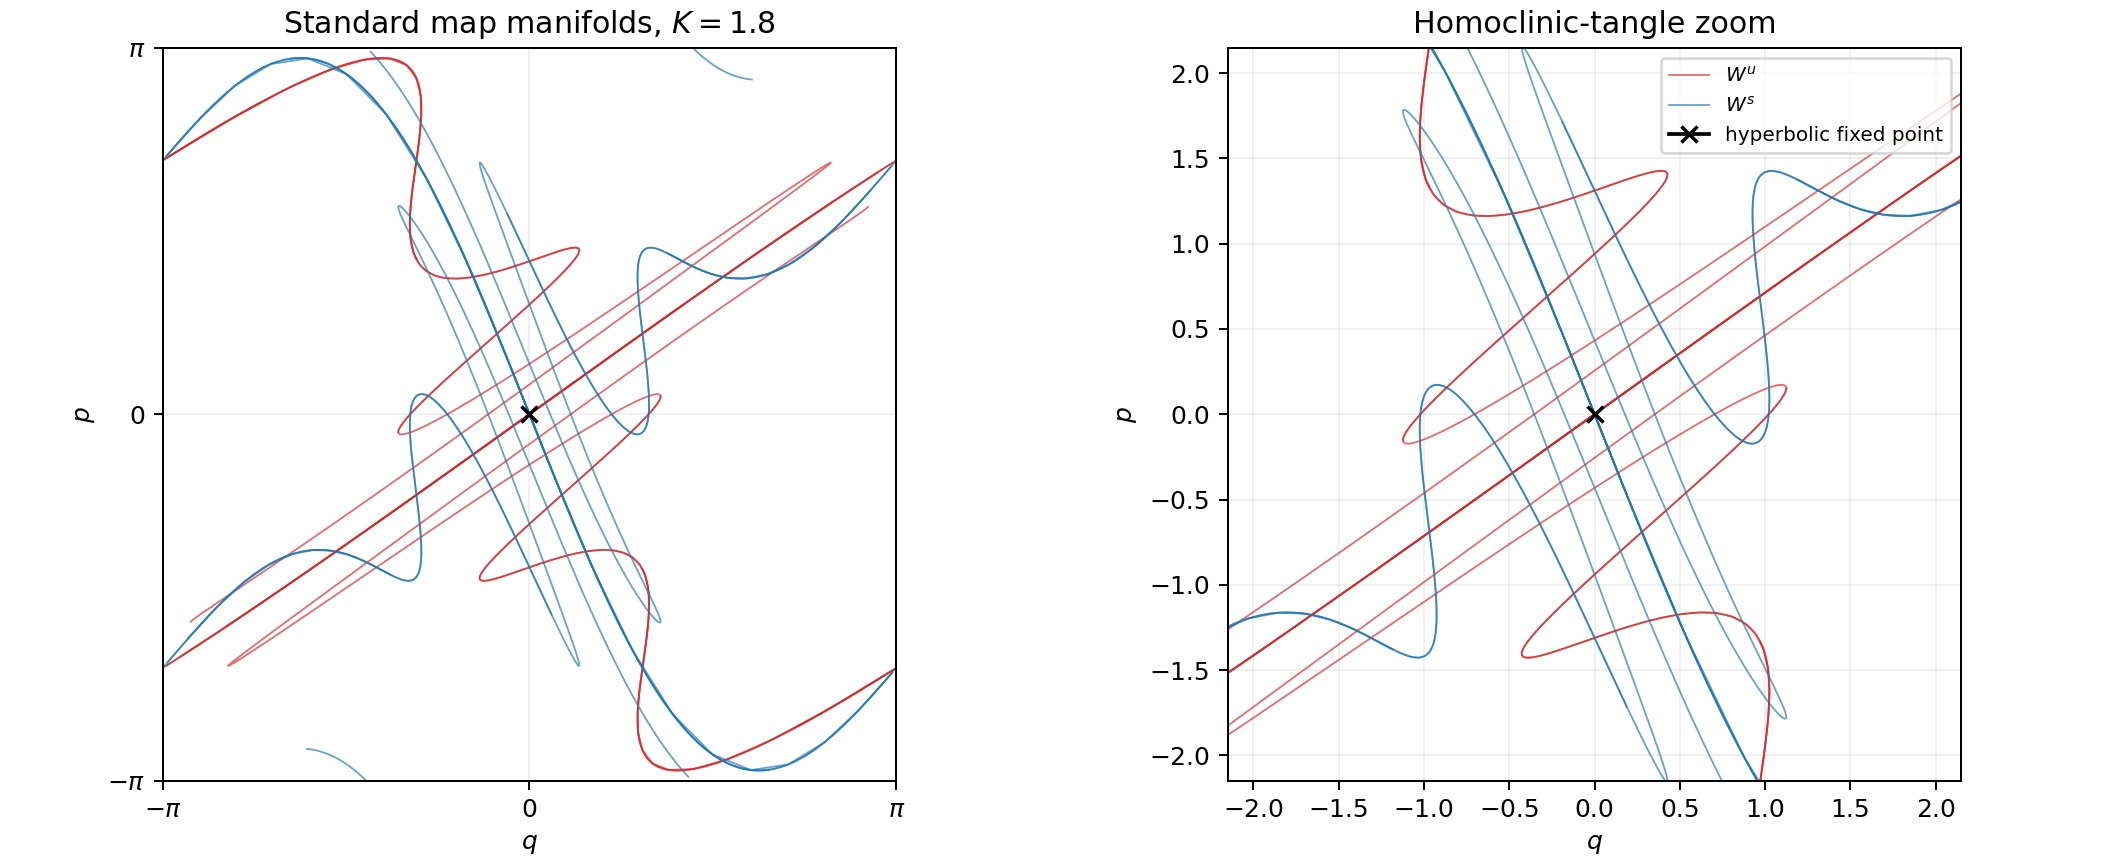
\includegraphics[width=0.98\textwidth]{../../figures/canonical/standard_map_homoclinic_tangle_quick.png}
\caption{Stable and unstable manifolds for the hyperbolic fixed point
\((q,p)=(0,0)\) of the standard map, generated by
\protect\path{demos/python/standard_map_homoclinic_tangle.py}.  Both panels use
the centered torus coordinates \((q,p)\in[-\pi,\pi)\times[-\pi,\pi)\), and the
map is \(p_{n+1}=p_n+K\sin q_n,\ q_{n+1}=q_n+p_{n+1}\) modulo \(2\pi\), with
\(K=1.8\) chosen so the splitting and folds are visible at lecture-note scale.
The black cross is the hyperbolic fixed point.  The red curves approximate
\(W^u\), the unstable manifold, by forward iterates of a tiny segment tangent
to the unstable eigenvector of the linearized map.  The blue curves approximate
\(W^s\), the stable manifold, by inverse iterates of a tiny segment tangent to
the stable eigenvector.  The left panel shows the computed manifold branches on
the torus; the right panel restricts the view to a smaller square so the
transverse red-blue crossings and folds of the homoclinic tangle are easier to
see.  These are finite numerical images of local tangent segments, not a
complete global parametrization of \(W^s\cup W^u\).}
\label{fig:standard-map-homoclinic-tangle}
\end{figure}

\subsection{Cantori And Partial Barriers}
\label{subsec:cantori-partial-barriers}

For area-preserving maps, the strongest irrational invariant curves are often
those whose rotation numbers are hardest to approximate by rationals. The
golden-mean rotation number
\[
  \rho_g=\frac{\sqrt5-1}{2}
\]
is the standard example because its continued fraction is
\([1;1,1,1,\ldots]\), making it maximally poorly approximated among
irrationals in the precise sense of Hurwitz's theorem: every irrational \(x\) has
infinitely many rationals \(p/q\) with
\[
  \left|x-\frac pq\right|<\frac{1}{\sqrt5\,q^2},
\]
and the constant \(\sqrt5\) is sharp, with equality approached by the golden
ratio and its fractional-linear equivalents.

When an irrational invariant curve finally breaks, Aubry-Mather theory
(Mather, 1982; Aubry, 1983) supplies the replacement object. For an
area-preserving twist map and an irrational
rotation number \(\rho\), there is an invariant Aubry-Mather set with rotation
number \(\rho\). If the KAM curve survives, this set is the curve itself. If
the curve has broken, the set is a Cantor-like invariant set called a
cantorus. Its gaps prevent it from being a continuous barrier, but small gaps
can still make transport through the associated turnstile lobes very slow.
This existence-and-order statement is a separate variational theorem, not a
consequence of KAM: KAM proves persistence of sufficiently nonresonant smooth
curves under small perturbations, while Aubry-Mather theory constructs ordered
minimizing orbits even after the smooth curve has broken.
One variational model is the Frenkel-Kontorova form of an exact twist map:
orbits are critical sequences of an action
\[
  \mathcal S(\{\theta_n\})=\sum_n L(\theta_n,\theta_{n+1}),
\]
with a prescribed mean rotation number. Minimizing sequences with irrational
rotation number are ordered and cannot cross. When the invariant curve exists,
these minimizers fill it; after breakup, the same ordered minimizers survive
only on a Cantor set.

For the standard map, a famous numerical benchmark is that the last invariant
curve with golden-mean rotation breaks near
\[
  K_c\approx0.971635.
\]
This number is obtained by numerical criteria such as Greene's 1979 residue
criterion, later sharpened by MacKay's renormalization work. For a rational
periodic orbit of period \(q\), the residue of the
\(q\)-fold derivative is
\[
  R=\frac{2-\tr(DT_K^q)}{4}.
\]
For an elliptic periodic point \(0<R<1\); for a hyperbolic point \(R<0\) or
\(R>1\). Greene's residue conjecture remains a conjecture: it says that an
irrational invariant curve
with rotation number \(\rho\) exists precisely when the residues of periodic
orbits whose rotation numbers \(p_n/q_n\) approach \(\rho\) remain bounded in
the appropriate limiting sense. The number \(K_c\approx0.971635\) is the value
at which this criterion predicts breakdown of the golden-mean invariant curve
in the standard map. Direct numerical simulations and MacKay-Stark style
renormalization results support the criterion in important cases, but it should
not be read as a proved theorem in the generality of its numerical use.

\begin{figure}[htbp]
\centering
\begin{tikzpicture}[scale=0.95, >=Latex, font=\small]
  \begin{scope}[shift={(0,0)}]
    \draw[->] (-0.2,0) -- (2.7,0) node[right] {\(\theta\)};
    \draw[->] (0,-0.15) -- (0,2.2) node[above] {\(J\)};
    \foreach \y/\amp in {0.45/0.04,0.85/0.06,1.25/0.05,1.65/0.04}
      \draw[blue!70!black, thick, domain=0.15:2.45, samples=80]
        plot (\x,{\y+\amp*sin(220*\x)});
    \draw[red!75!black, thick, ->] (0.55,0.63) -- (1.45,0.63);
    \node[align=center, text width=2.8cm] at (1.35,-0.70)
      {surviving invariant curves block crossing};
  \end{scope}

  \begin{scope}[shift={(4.0,0)}]
    \draw[->] (-0.2,0) -- (2.7,0) node[right] {\(\theta\)};
    \draw[->] (0,-0.15) -- (0,2.2) node[above] {\(J\)};
    \foreach \x in {0.55,1.35,2.15}
    {
      \draw[orange!85!black, thick] (\x,1.05) ellipse (0.28 and 0.17);
      \fill[orange!85!black] (\x,1.05) circle (1.1pt);
    }
    \foreach \x in {0.95,1.75}
    {
      \draw[purple!75!black, thick] (\x-0.10,0.95) -- (\x+0.10,1.15);
      \draw[purple!75!black, thick] (\x-0.10,1.15) -- (\x+0.10,0.95);
    }
    \draw[purple!65!black, densely dashed]
      (0.10,1.05) .. controls (0.55,1.55) and (1.05,1.55) .. (1.35,1.23)
      .. controls (1.70,1.55) and (2.20,1.55) .. (2.55,1.05);
    \draw[purple!65!black, densely dashed]
      (0.10,1.05) .. controls (0.55,0.55) and (1.05,0.55) .. (1.35,0.87)
      .. controls (1.70,0.55) and (2.20,0.55) .. (2.55,1.05);
    \node[align=center, text width=2.8cm] at (1.35,-0.70)
      {rational curve becomes islands and saddles};
  \end{scope}

  \begin{scope}[shift={(8.0,0)}]
    \draw[->] (-0.2,0) -- (2.7,0) node[right] {\(\theta\)};
    \draw[->] (0,-0.15) -- (0,2.2) node[above] {\(J\)};
    \draw[blue!70!black, thick, domain=0.15:0.65, samples=30]
      plot (\x,{1.05+0.05*sin(240*\x)});
    \draw[blue!70!black, thick, domain=0.86:1.36, samples=30]
      plot (\x,{1.05+0.05*sin(240*\x)});
    \draw[blue!70!black, thick, domain=1.58:2.28, samples=40]
      plot (\x,{1.05+0.05*sin(240*\x)});
    \draw[red!75!black, thick, fill=red!10]
      (0.68,0.72) .. controls (0.86,0.88) and (0.86,1.12) .. (1.05,1.25)
      .. controls (0.90,1.12) and (0.86,0.93) .. (0.68,0.72);
    \draw[red!75!black, thick, fill=red!10]
      (1.42,1.36) .. controls (1.58,1.22) and (1.56,0.96) .. (1.78,0.82)
      .. controls (1.62,0.96) and (1.58,1.15) .. (1.42,1.36);
    \draw[red!75!black, thick, ->] (0.76,0.82) .. controls (0.87,0.95) .. (0.98,1.08);
    \draw[red!75!black, thick, ->] (1.50,1.26) .. controls (1.60,1.12) .. (1.70,0.98);
    \foreach \x/\y in {0.78/1.48,1.72/0.58}
      \fill[red!75!black] (\x,\y) circle (1.2pt);
    \draw[red!75!black, ->, thick] (0.78,1.48) -- (0.92,1.28);
    \draw[red!75!black, ->, thick] (1.72,0.58) -- (1.58,0.78);
    \foreach \x/\y in {0.72/1.02,1.46/1.08,2.20/1.05}
      \draw[blue!70!black, fill=white, thick] (\x,\y) circle (1.1pt);
    \node[align=center, text width=2.8cm] at (1.35,-0.70)
      {cantorus leaves gaps and slow turnstiles};
  \end{scope}
\end{tikzpicture}
\caption{Three stages in the loss of transport barriers on a two-dimensional
section. Left: invariant curves separate the annulus. Middle: a rational curve
splits into an island chain with hyperbolic points. Right: an irrational curve
may leave a cantorus, which permits transport only through gaps.}
\label{fig:torus-breakdown-stages}
\end{figure}

The accompanying Python script
\path{demos/python/standard_map_torus_breakdown.py} uses the standard map on
the cylinder. It initializes an ensemble near the golden-mean unperturbed
rotation number, leaves \(p\) unwrapped, and measures finite-time momentum
spreading. A large spread is evidence of transport through broken barriers; a
small spread over finite time is not a proof of survival. The corresponding
Makefile target is \path{standard-map-breakdown-demo}, and the Wolfram
Language companion is
\path{demos/mathematica/StandardMapTorusBreakdown.wl}. This distinction is
essential: numerical trajectories illustrate the geometry, while KAM,
Poincare-Birkhoff theory, and separatrix-splitting criteria explain why the
geometry is there.

\section{From Resonance To Chaos: Poincare Map Picture}
\label{sec:poincare-resonance-chaos}

A Poincare section converts continuous Hamiltonian motion into an
area-preserving map. This loses the time parametrization but keeps the geometry
needed to see resonance. Near a resonant torus, some iterate of the unperturbed
map is the identity; after perturbation, that near-identity map unfolds into
fixed points, island chains, and separatrices.
Poincare introduced this return-map viewpoint in the \emph{Methodes nouvelles};
it is one of the reasons that modern Hamiltonian chaos is usually drawn on a
section before it is described in full phase space.

\paragraph{Local notation.}
The section \(S\) below is a transverse surface inside a fixed energy surface,
and \(T:S\to S\) is the first-return map.  The symbol \(T\) in this section is
a map, not kinetic energy.  The iterate \(T^q\) means applying the return map
\(q\) times.

This is why maps are so useful in a chapter about flows. A continuous orbit can
hide its organization in time; a section records each return to a transverse
surface and turns invariant tori into curves, resonances into island chains,
and chaotic layers into visible scatter. The standard map isolates this
return-map geometry in its simplest widely used form.

For two degrees of freedom, begin with an integrable Hamiltonian
\[
  H_0=H_0(I_1,I_2),
  \qquad
  (I_1,I_2,\theta_1,\theta_2)\in U\times\mathbb T^2,
\]
and fix an energy surface \(H_0=E\). Choose a Poincare section \(S\), for
example \(\theta_2=0\). Starting from \(x\in S\), follow the orbit until it
next intersects \(S\). This defines the return map
\[
  T:S\to S.
\]
The unperturbed flow has
\[
  \dot\theta_1=\omega_1(I),
  \qquad
  \dot\theta_2=\omega_2(I).
\]
Returning to \(\theta_2=0\) takes time \(2\pi/\omega_2\), so the return map
twists the remaining angle by
\[
  \Delta\theta_1=2\pi\frac{\omega_1}{\omega_2}.
\]
On a resonant torus with \(\omega_1/\omega_2=p/q\),
\[
  T^q=\id
\]
for the unperturbed return map \(T\). A concrete period-three resonance is
\[
  \frac{\omega_1}{\omega_2}=\frac13,
  \qquad
  T:\theta_1\mapsto\theta_1+\frac{2\pi}{3},
  \qquad
  T^3=\id.
\]
Let \(C\subset S\) be the invariant curve obtained by intersecting this
resonant torus with the section. Nearby invariant curves \(C_-\) and \(C_+\)
have slightly different rotation numbers. With the twist condition
\(\dd\Omega/\dd I\neq0\), \(T^3\) rotates points one way on \(C_-\) and the
opposite way on \(C_+\).

Now perturb the Hamiltonian:
\[
  H=H_0+\eps H_1.
\]
The perturbed Poincare map \(T_\eps\) is still defined by first return to
\(S\), even though the invariant tori may no longer exist. Near
\(C\cap S\), \(T_\eps^3\) is close to the identity. At fixed energy it has the
local form
\[
  T_\eps^3(I_1,\theta_1)
  =
  \left(
    I_1+f_\eps(I_1,\theta_1),
    \theta_1+g_\eps(I_1,\theta_1)
  \right).
\]
For small \(\eps\), the opposite twists on \(C_-\) and \(C_+\) persist.
Therefore an intermediate curve \(C'\) has
\[
  g_\eps(I_1,\theta_1)=0;
\]
on \(C'\), the third-return map produces no angular displacement.

The missing radial displacement is controlled by area preservation. Hamiltonian
flow preserves \(\omega\), and hence the Poincare map preserves the induced
area form on the section. Equivalently, for a closed curve \(\gamma\) bounding
a disk \(D_\gamma\) in the section,
\[
  \oint_\gamma p\,\dd q
  =
  -\int_{D_\gamma}\omega,
\]
so the signed symplectic area enclosed by \(\gamma\) is invariant. If
\(f_\eps\) were nonzero with a fixed sign everywhere on \(C'\), the curve
would be displaced monotonically inward or outward under \(T_\eps^3\), changing
the enclosed area. Thus \(f_\eps\) must have at least a pair of zeros on
\(C'\). At such points
\[
  f_\eps=0,
  \qquad
  g_\eps=0,
\]
so \(T_\eps^3\) has fixed points. In the period-three example, if \(x\) is a
fixed point of \(T_\eps^3\), then \(T_\eps(x)\) is also a fixed point of
\(T_\eps^3\). Thus the resonant curve generically produces six fixed points:
three elliptic and three hyperbolic, alternating around the resonant layer.

Elliptic points are surrounded by island chains and new local invariant curves.
Hyperbolic points have stable and unstable manifolds. Once those manifolds
intersect transversely, the separatrix is replaced by a chaotic layer. Farther
from the resonance, sufficiently Diophantine KAM curves persist and confine
motion.

This is the local mechanism behind the pictures one sees in the standard map,
the driven pendulum, and the asteroid-belt resonances: KAM tori survive away
from strong resonances, while resonant tori break into islands and chaotic
separatrix webs.
For the real asteroid belt, this local statement is only the beginning of a
quantitative model. Resonance widths, eccentricity dependence, secular
precession, and close encounters require the celestial variables of the
restricted three-body problem rather than the single-pendulum normal form alone.

\section{The Standard Map As A Minimal Model}
\label{sec:standard-map}

The standard map is
\[
\begin{aligned}
  p_{n+1} &= p_n+K\sin q_n,\\
  q_{n+1} &= q_n+p_{n+1}\pmod{2\pi}.
\end{aligned}
\]

\paragraph{Local notation.}
The integer \(n\) is an iterate label, \(K\) is the kick strength, \(q\) is an
angle, and \(p\) is the conjugate momentum-like coordinate of the map.  On the
cylinder \(p\) is real and unwrapped; on the compact two-torus portrait both
\(q\) and \(p\) are reduced modulo \(2\pi\).

This map is often called the Chirikov standard map. It emerged from kicked
rotor and resonance-overlap models in the 1960s, and Chirikov's 1979 review made
it the canonical laboratory for the transition from invariant curves to global
Hamiltonian chaos.
This is naturally a map of the cylinder, with \(q\) taken modulo \(2\pi\) and
\(p\in\R\). For phase portraits on a compact square, the Python demo reduces
both \(q\) and \(p\) modulo \(2\pi\), giving the corresponding map on the
two-torus.
It is area-preserving because the Jacobian matrix has determinant one:
\[
  D\Psi=
  \begin{pmatrix}
  1+K\cos q_n & 1\\
  K\cos q_n & 1
  \end{pmatrix},
  \qquad
  \det D\Psi=1.
\]
The parameter \(K\) controls resonance overlap. For small \(K\), invariant
curves dominate. For larger \(K\), chaotic regions grow.
The compact two-torus portrait is useful for seeing islands, but it hides
whether an orbit has crossed many momentum cells on the cylinder. For transport
questions one should keep \(p\) unwrapped; this is the convention used in the
torus-breakdown diagnostic demo.

\begin{example}[Period-three resonance in the standard map]
A common drift-kick convention for the standard map is
\[
  T_K(\theta,p)=\left(\theta+p,\ p+K\sin(\theta+p)\right),
\]
which is symplectically equivalent to the convention above after shifting where
the kick is placed. If
\[
  D(\theta,p)=(\theta+p,p),\qquad Kc(\theta,p)=(\theta,p+K\sin\theta),
\]
then the map used above is
\[
  D\circ Kc,
\]
whereas the drift-kick convention is
\[
  Kc\circ D.
\]
These differ by where the stroboscopic section is placed along the kicked flow;
the phase portraits and resonant normal forms are conjugate after this section
shift. At \(K=0\), the invariant curve
\[
  C:\quad p=\frac{2\pi}{3}
\]
has
\[
  T_0^3=\id
\]
because the angle advances by \(2\pi\) after three iterates.

Let
\[
  p=\frac{2\pi}{3}+\delta(\theta),
  \qquad
  \delta=O(K).
\]
To first order in \(K\) and \(\delta\),
\[
\begin{aligned}
  \theta_3-\theta-2\pi
  &=
  3\delta
  +
  2K\sin\left(\theta+\frac{2\pi}{3}\right)
  +
  K\sin\left(\theta+\frac{4\pi}{3}\right)
  +O(K^2),
\end{aligned}
\]
where \(\theta_3\) denotes the angle component after three iterates of
\(T_K\).
The nearby curve \(C'\) on which \(T_K^3\) fixes the angle therefore satisfies
\[
  \boxed{
  \delta(\theta)
  =
  \frac{K}{2}\sin\theta
  -
  \frac{K\sqrt3}{6}\cos\theta
  +
  O(K^2).
  }
\]
For example, at \(\theta=\pi/3\),
\[
  p=\frac{2\pi}{3}+\frac{K}{2\sqrt3}+O(K^2),
\]
which is the initial condition singled out in the corresponding numerical
exercise. At the next order, the area-preserving twist-map argument behind
Poincare-Birkhoff forces the radial displacement on \(C'\) to have alternating
zeros. These become the six period-three points: three elliptic island centers
and three hyperbolic points with separatrix structure.
\end{example}

\begin{figure}[htbp]
\centering
\begin{tikzpicture}
\begin{axis}[
  width=0.86\textwidth,
  height=0.64\textwidth,
  xmin=0, xmax=6.283185,
  ymin=0, ymax=6.283185,
  axis lines=left,
  axis line style={-Latex},
  xlabel={\(q\)},
  ylabel={\(p\)},
  xtick={0,1.570796,3.141593,4.712389,6.283185},
  xticklabels={\(0\),\(\pi/2\),\(\pi\),\(3\pi/2\),\(2\pi\)},
  ytick={0,2.094395,4.188790,6.283185},
  yticklabels={\(0\),\(2\pi/3\),\(4\pi/3\),\(2\pi\)},
  tick style={black},
  grid=both,
  major grid style={black!10},
  minor tick num=1,
  minor grid style={black!4},
  clip=true,
  legend style={
    at={(0.5,-0.16)},
    anchor=north,
    legend columns=2,
    draw=none,
    fill=white,
    font=\scriptsize,
    /tikz/every even column/.append style={column sep=0.35cm}
  },
  legend image post style={mark size=1.2pt},
]
  \addplot[only marks, mark=*, mark size=0.23pt, blue!45]
    table[x=q,y=p] {data/standard_map_kam_K065.dat};
  \addlegendentry{quasiperiodic curves}
  \addplot[only marks, mark=*, mark size=0.30pt, black!38]
    table[x=q,y=p] {data/standard_map_period3_layer_K065.dat};
  \addlegendentry{separatrix layer}
  \addplot[only marks, mark=*, mark size=0.32pt, red!65!black]
    table[x=q,y=p] {data/standard_map_period3_islands_K065.dat};
  \addlegendentry{period-three islands}
  \addplot[densely dashed, black!45]
    coordinates {(0,2.094395) (6.283185,2.094395)};
  \addplot[only marks, mark=*, mark size=1.45pt, red!75!black]
    coordinates {(0.880179,1.760359) (3.141593,2.261413) (5.403006,2.261413)};
  \addplot[only marks, mark=x, mark size=3.0pt, line width=0.8pt, purple!75!black]
    coordinates {(0.000000,1.888577) (1.888577,1.888577) (4.394609,2.506032)};
  \addlegendentry{hyperbolic points}
  \node[anchor=west, black!55, fill=white, inner sep=1pt] at (axis cs:5.10,2.76)
    {\(p=2\pi/3\)};
\end{axis}
\end{tikzpicture}
\caption{Actual iterates of the standard map on the compact two-torus at
\(K=0.65\).  Both axes are angles modulo \(2\pi\): the horizontal coordinate
is \(\theta\) and the vertical coordinate is \(p\), plotted in the square
\([0,2\pi)\times[0,2\pi)\).  Each dot is one iterate of
\(p_{n+1}=p_n+K\sin\theta_n,\ \theta_{n+1}=\theta_n+p_{n+1}\), reduced modulo
\(2\pi\). Blue points lie on quasiperiodic invariant curves away from the
resonance, red points trace orbits near the elliptic period-three island chain,
gray points sample the local separatrix layer, and purple crosses mark the
hyperbolic period-three orbit.  The dashed line \(p=2\pi/3\) is a reference
line for the resonant rotation number, not a trajectory.}
\label{fig:standard-map-island-chain}
\end{figure}

\section{What To Take Forward}
\label{sec:perturbation-chaos-take-forward}

The main logical chain of this chapter is the following. Complete
integrability gives invariant tori carrying quasi-periodic motion. In
action-angle variables an integrable Hamiltonian depends only on the actions,
so the frequencies are gradients of \(H_0(I)\). A small perturbation introduces
angle-dependent terms. Canonical perturbation theory tries to remove those
terms order by order, but the homological equation divides by integer
frequency combinations \(k\cdot\omega(I)\). Small divisors are the obstruction
that distinguishes robust quasi-periodic motion from resonant dynamics.

KAM theory says that sufficiently nonresonant tori with nondegenerate frequency
maps survive the small analytic perturbations considered in this chapter,
though the tori deform. Resonant tori are more fragile. Near resonance, the
averaged dynamics reduces to pendulum-like islands, separatrices, and
stochastic layers. As perturbations grow, resonance overlap destroys transport
barriers and produces large chaotic regions.

The standard map is a minimal laboratory where these stages can be seen in one
picture: rotational invariant curves at small coupling, island chains around
rational rotation numbers, cantori and partial barriers near the breakup
threshold, and widespread diffusion when barriers are gone.

For asteroid resonances, the same pendulum geometry becomes quantitative only
after a disturbing-function coefficient is computed. The \(2:1\) calculation
in this chapter is the first such coefficient-level bridge between the formal
normal form and the numerical asteroid experiments.

The three-body problem in Chapter~\ref{chap:three-body-problem} is a principal
physical arena for these ideas. It is not included here because its Newtonian
reduction, restricted limit, Lagrange points, and asteroid-belt ensembles
deserve a self-contained treatment.

\section{Chapter-End Laboratories And Exercises}
\label{sec:perturbation-chaos-chapter-end-labs}

The laboratories below are finite-dimensional tests of the perturbative logic:
slow resonant angles, pendulum normal forms, small divisors, island chains, and
the onset of chaotic regions.

\subsection{Driven One-Angle Hamiltonian And Resonant Normal Form}
\label{sec:detailed-driven-resonance}

Consider the one-angle time-periodic perturbation model
\[
  H(I,\theta,t)
  =
  \frac12I^2+\epsilon\cos(n\theta-\nu t).
\]

\paragraph{Local notation.}
In this exercise \(I\) is the action conjugate to the angle \(\theta\), the
integer \(n\) labels the harmonic in the perturbation, and \(\nu\) is the
external driving frequency.  The variable \(E_t\) introduced below is the
momentum conjugate to time in the autonomous extended phase space.

The unperturbed frequency is
\[
  \dot\theta=I.
\]
Resonance occurs when the phase
\[
  \psi=n\theta-\nu t
\]
is slow, i.e.
\[
  nI-\nu\approx0.
\]
Thus
\[
  I_{\mathrm{res}}=\frac{\nu}{n}.
\]
To make the system autonomous, introduce the extended phase-space pair
\((t,E_t)\), with Hamiltonian
\[
  K=E_t+\frac12I^2+\epsilon\cos(n\theta-\nu t).
\]
Use the type-II generating function
\[
  F_2(\theta,t;J,\mathcal E)
  =
  (n\theta-\nu t)J+t\mathcal E.
\]
It gives
\[
  \psi=\frac{\partial F_2}{\partial J}=n\theta-\nu t,
  \qquad
  \tau=\frac{\partial F_2}{\partial \mathcal E}=t,
\]
and
\[
  I=\frac{\partial F_2}{\partial\theta}=nJ,
  \qquad
  E_t=\frac{\partial F_2}{\partial t}=-\nu J+\mathcal E.
\]
Thus the autonomous Hamiltonian becomes, up to the spectator variable
\(\mathcal E\),
\[
  K'=\mathcal E-\nu J+\frac12n^2J^2+\epsilon\cos\psi.
\]
The resonance condition is
\[
  \frac{\partial K'}{\partial J}=-\nu+n^2J=0,
\]
so
\[
  J_{\mathrm{res}}=\frac{\nu}{n^2},
  \qquad
  I_{\mathrm{res}}=nJ_{\mathrm{res}}=\frac{\nu}{n}.
\]
Set
\[
  J=J_{\mathrm{res}}+P.
\]
After dropping constants and the decoupled \(\mathcal E\), the resonant
Hamiltonian is
\[
  \boxed{
  K_{\mathrm{res}}(P,\psi)
  =
  \frac12 n^2P^2+\epsilon\cos\psi.
  }
\]
This is a pendulum Hamiltonian with effective inverse mass \(n^2\). It has
elliptic islands, hyperbolic fixed points, and a separatrix. This is why
planetary mean-motion resonances, the standard map, and the driven pendulum
share the same local geometry.

\subsection{Henon-Heiles As The Finite-Dimensional Chaos Bridge}
\label{sec:lab-henon-heiles}

Henon and Heiles introduced this Hamiltonian in 1964 as a galactic-dynamics
model, and it became one of the first smooth Hamiltonian systems where
numerical Poincare sections made the breakdown of integrability visible. The
Henon-Heiles Hamiltonian is
\[
  H_{\mathrm{HH}}
  =
  H_0+\lambda_{\mathrm{HH}}H_1,
\]

\paragraph{Local notation.}
The phase-space coordinates are \((x,y,p_x,p_y)\).  The parameter
\(\lambda_{\mathrm{HH}}\) controls the nonlinear perturbation and is written
with a subscript to avoid confusion with the angle \(\lambda\) used in
celestial mechanics.  The Poincare sections later in the exercise fix one
coordinate and plot the remaining conjugate pair at each crossing.

with
\[
  H_0=
  \frac12(p_x^2+p_y^2+x^2+y^2),
  \qquad
  H_1=x^2y-\frac13y^3.
\]
For the isotropic oscillator, introduce action-angle variables
\[
  x=\sqrt{2I_1}\sin\theta_1,
  \qquad
  p_x=\sqrt{2I_1}\cos\theta_1,
\]
\[
  y=\sqrt{2I_2}\sin\theta_2,
  \qquad
  p_y=\sqrt{2I_2}\cos\theta_2.
\]
Then
\[
  H_0=I_1+I_2,
  \qquad
  \omega_0=(1,1).
\]
The first-order homological equation for a generating function \(S_1\) is
\[
  \omega_0\cdot\partial_\theta S_1
  =
  \langle H_1\rangle-H_1.
\]
In Fourier components,
\[
  i(k_1+k_2)S_{1k}=-H_{1k}.
\]
The denominator vanishes whenever
\[
  k_1+k_2=0.
\]
At first order the cubic perturbation has no average and its Fourier expansion
contains no nonzero mode with \(k_1+k_2=0\). The first-order homological
equation can therefore be solved for all modes that appear. At second order,
however, the canonical transformation generates resonant Fourier modes with
\(k_1+k_2=0\). Those modes cannot be removed by a periodic \(S_2\). This is the
small-divisor obstruction in its most concrete classroom form: the unperturbed
oscillator has equal frequencies, so resonant combinations of angles do not
average away.
For example, the second-order transformed Hamiltonian contains
\[
  \frac{\lambda_{\mathrm{HH}}^2}{2}\{H_1,S_1\}.
\]
Products of first-order Fourier modes add their wave vectors. Nonresonant
modes \(k\) and \(k'\) in \(H_1\) can therefore produce combinations such as
\(k+k'=(2,-2)\), which satisfy \((k+k')\cdot\omega_0=0\). The obstruction is
not that the first-order cubic term is already resonant; it is that the
near-identity transformation creates resonant terms at the next order.

The Henon-Heiles system is a useful finite-dimensional bridge from
integrability to Hamiltonian chaos. At low energy, Poincare sections show
deformed invariant curves. At higher energy, resonance islands and chaotic
regions appear. Unlike the asteroid problem, all variables and forces remain
visible in a four-dimensional phase space.

\begin{figure}[htbp]
\centering
\begin{tikzpicture}
\begin{axis}[
  name=hhlow,
  width=0.46\textwidth,
  height=0.46\textwidth,
  xmin=-0.55, xmax=0.55,
  ymin=-0.55, ymax=0.55,
  axis equal image,
  axis lines=left,
  axis line style={-Latex},
  xlabel={\(x\)},
  ylabel={\(p_x\)},
  title={\(E=1/12\)},
  tick style={black},
  grid=both,
  major grid style={black!10},
  minor tick num=1,
  minor grid style={black!4},
  clip=true,
]
  \addplot[only marks, mark=*, mark size=0.10pt, blue!55!black]
    table[x=x,y=px] {data/henon_heiles_section_E083333.dat};
  \addplot[densely dashed, red!70!black, domain=0:360, samples=180, variable=\t]
    ({0.4082482905*cos(\t)}, {0.4082482905*sin(\t)});
\end{axis}
\begin{axis}[
  at={(hhlow.east)},
  anchor=west,
  xshift=0.45cm,
  width=0.46\textwidth,
  height=0.46\textwidth,
  xmin=-0.55, xmax=0.55,
  ymin=-0.55, ymax=0.55,
  axis equal image,
  axis lines=left,
  axis line style={-Latex},
  xlabel={\(x\)},
  ylabel={\(p_x\)},
  title={\(E=1/8\)},
  tick style={black},
  grid=both,
  major grid style={black!10},
  minor tick num=1,
  minor grid style={black!4},
  clip=true,
]
  \addplot[only marks, mark=*, mark size=0.10pt, black!52]
    table[x=x,y=px] {data/henon_heiles_section_E125000.dat};
  \addplot[densely dashed, red!70!black, domain=0:360, samples=180, variable=\t]
    ({0.5000000000*cos(\t)}, {0.5000000000*sin(\t)});
\end{axis}
\end{tikzpicture}
\caption{Numerical Poincare sections of the Henon-Heiles flow on
\(y=0,\ p_y>0\), generated from the data files written by
\protect\path{demos/python/henon_heiles_poincare.py}.  In each panel the horizontal
axis is \(x\) and the vertical axis is \(p_x\), both in the nondimensional
units of the Hamiltonian in the text.  The integration records one point each
time the orbit crosses the section upward; \(p_y\) is then determined by the
fixed energy and is not an independent plotted coordinate.  The dashed red
circle is the kinematic boundary \(x^2+p_x^2=2E\) on the section, where
\(p_y=0\). At \(E=1/12\) the section is dominated by deformed invariant
curves; by \(E=1/8\) a chaotic sea coexists with surviving islands and smaller
regular regions.}
\label{fig:lab-henon-heiles}
\end{figure}
\FloatBarrier

\subsection{Questions For The Reader}
\label{sec:perturbation-chaos-questions}

\begin{enumerate}
\item In the homological equation
\(\omega(I)\cdot\partial_\theta S_1=-(H_1-\langle H_1\rangle)\), identify
where the Diophantine condition is used. What fails if \(\omega\) is
rational?
\item For a one-degree-of-freedom resonant normal form, draw the phase portrait
and identify elliptic fixed points, hyperbolic fixed points, separatrices, and
island width. Which part of this picture persists in an area-preserving map?
\item Use the standard-map figure in this chapter to compare three types of
phase-space organization: invariant curves, resonance islands, and chaotic
layers. Which of these can block global radial transport in action?
\item Explain why Liouville volume preservation is compatible with chaos. Which
property of the dynamics changes when invariant tori break?
\item In Figure~\ref{fig:asteroid-resonance-normal-form-numerical}, identify
which curve is a genuine \(2:1\) disturbing-function calculation and which
curves are order-of-eccentricity scaling models.  How would the half-width
change if Jupiter's mass were multiplied by \(25\)?
\end{enumerate}

\section{Associated Demos}
\label{sec:perturbation-chaos-demos}

The associated torus-breakdown and finite-dimensional chaos demos are:
\begin{itemize}
\item \path{demos/python/asteroid_resonance_normal_form.py}
\item \path{demos/python/standard_map_homoclinic_tangle.py}
\item \path{demos/python/standard_map_torus_breakdown.py}
\item \path{demos/python/henon_heiles_poincare.py}
\item \path{demos/mathematica/StandardMapTorusBreakdown.wl}
\end{itemize}
They reproduce the transition from invariant curves to resonance islands and
chaotic layers.  The asteroid normal-form script also computes the \(2:1\)
disturbing-function coefficient and the corresponding width estimate, so the
chapter contains both a universal pendulum model and one coefficient-level
celestial calculation.
